\documentclass[a4paper,14pt,oneside,openany]{memoir}
\usepackage[left=2.5cm, right=1cm, top=2cm, bottom=2cm]{geometry}

\usepackage[backend=biber,style=numeric,sorting=none]{biblatex}
\DeclareFieldFormat{labelnumberwidth}{{#1\adddot}}
  
\usepackage{bm}
\usepackage{amsmath}
\usepackage[russian]{babel}
\renewcommand{\baselinestretch}{1.5}
\setlength{\parindent}{1.25cm}
\usepackage{indentfirst}
\usepackage[utf8]{inputenc}
\usepackage{csquotes}

%% pics
\usepackage{graphicx}
\usepackage{caption}
\captionsetup[figure]{name={Рисунок}}
\graphicspath{ {./pics/} }

%% sections style
\usepackage{titlesec}
\titleformat*{\section}{\normalfont\bfseries}

%% page style
\pagestyle{myheadings} % нумерация страниц вверху справа
\aliaspagestyle{chapter}{myheadings} % нумерация страниц вверху справа
\renewcommand{\cftchapterpagefont}{\normalfont}% нежирные номера страниц у глав в оглавлении
\renewcommand{\cftchapterleader}{\cftdotfill{\cftchapterdotsep}}% нежирные точки до номеров страниц у глав в оглавлении
\renewcommand{\cftchapterfont}{}% нежирные названия глав в оглавлении

\addbibresource{bibliography/citations.bib}

\begin{document}
	\thispagestyle{empty}
\begin{center} 
«Федеральное государственное автономное образовательное учреждение высшего образования «Московский физико-технический институт (национальный исследовательский университет)»
\end{center}
\begin{center} 
Физтех-школа Аэрокосмических Технологий
\end{center}

{
   	\vskip 5mm
}

\begin{flushleft}
\textbf{Направление подготовки:} 24.06.01 Авиационная и ракетно-космическая техника

\textbf{Направленность (профиль) подготовки:} 05.07.09 Динамика, баллистика, управление движением летательных аппаратов

\textbf{Форма обучения:} очная
\end{flushleft}

{
	\vskip 1cm
}

\begin{center} 
\textbf{НАУЧНЫЙ ДОКЛАД ОБ ОСНОВНЫХ РЕЗУЛЬТАТАХ ПОДГОТОВЛЕННОЙ НАУЧНО-КВАЛИФИКАЦИОННОЙ РАБОТЫ (ДИССЕРТАЦИИ)}
\end{center}

\begin{center} 
\textbf{«Анализ динамики и разработка методов управления движением квадрокоптера с поворотными роторами»}
\end{center}

{
	\vskip 1cm
}


\begin{flushright}
\textbf{Aспирант:} Шавин Михаил Юрьевич \hspace{16mm} \vspace{5mm}

$\rule{5cm}{0.15mm}$

\textbf{Научный руководитель:}  \hspace{41mm}

Притыкин Дмитрий Аркадьевич, к.ф.-м.н., \hspace{6mm} 

ст. науч. сотр. Космического центра Сколтеха \vspace{5mm}

$\rule{5cm}{0.15mm}$

\end{flushright}

{
	\vskip 5mm
}

\begin{center} 
Москва 2019
\end{center}

	\tableofcontents
	
\chapter{Общая характеристика работы}

\section{Актуальность темы исследования}

Беспилотные летательные аппараты (БЛА) мультироторного типа находят все более широкое применение в различных областях деятельности, а миниатюризация и доступность электронных компонентов их бортового оборудования приводит к расширению спектра задач, в решении которых используются такие аппараты.

С момента создания первых квадрокоптеров интенсивно ведутся исследования в области их динамики и управления, причем количество работ растет с каждым годом, что можно наблюдать по динамике количества публикаций (рис. \ref{pic:res_amount}), посвященных квадрокоптерам, доступных на крупнейшей онлайн платформе научных публикаций «Google Академия».

\begin{figure}[h!]
	\centering
	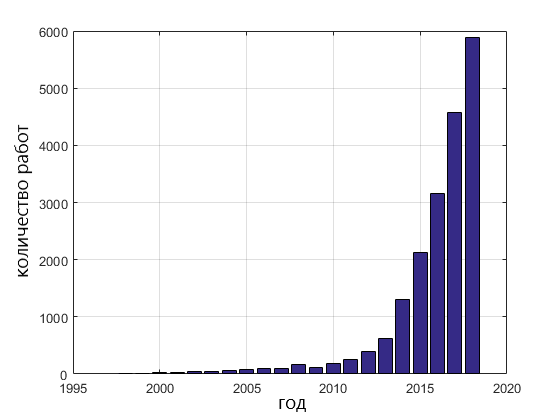
\includegraphics[width=0.75\columnwidth]{res_amount}
	\caption{ -- Динамика количества публикаций, посвященных квадрокоптерам}
	\label{pic:res_amount}
\end{figure}

Однако, несмотря на обилие публикаций в области управляемой динамики квадрокоптеров, остаются перспективные направления, среди которых усовершенствование конструкции БЛА, связанное с увеличением размерности вектора управляющих воздействий.
Конструктивно это достигается, например, с помощью сервоприводов, способных поворачивать роторы с пропеллерами относительно корпуса.

Стандартный квадрокоптер с четырехмерным вектором управляющих воздействий и шестью степенями свободы корпуса аппарата не способен, например, независимо управлять положением и ориентацией.
Это приводит к необходимости дополнительных устройств для наведения камер или лазерных дальномеров, используемых при выполнении ряда стандартных для БЛА задач.
Возможность независимо управлять положением и ориентацией, приобретаемая за счет использования поворотных роторов, влияет не только на работу полезной нагрузки и датчиков, но и на функциональные возможности всей системы в целом.
Усовершенствованные таким образом квадрокоптеры более устойчивы к возмущениям внешней среды, а также лучше стандартных квадрокоптеров пригодны для вертикального взлета и посадки на неровные поверхности.
Достоинства БЛА с поворотными роторами отмечают и исследователи, работающие над управлением БЛА в экстренных ситуациях (при отказе части двигателей).
В некоторых работах обосновывается достижение более высокой скорости за счет выбора оптимальной по отношению к набегающему потоку ориентации, а также более рациональное, по сравнению со стандартными аппаратами, энергопотребление.

\section{Цели и задачи исследования}

Объектом исследования является система управления движением квадрокоптера с поворотными роторами, предметом исследования -- динамика и методы управления движением квадрокоптера с поворотными роторами.

Цель работы -- исследовать динамику квадрокоптера с поворотными роторами;
разработать алгоритмы управления движением квадрокоптера с поворотными роторами для выполнения различных маневров;
разработать алгоритмы экстренного управления движением квадрокоптера с поворотными роторами.
Для достижения цели работы необходимо решить следующие задачи:
\begin{enumerate}
	\item Разработать математическую модель движения квадрокоптера с поворотными роторами с учетом сил и моментов, действующих на все составные части системы.
	\item Решить задачу обратной динамики и синтезировать контур управления квадрокоптером с поворотными роторами для независимого управления положением и ориентацией аппарата с учетом физических ограничений, накладываемых на исполнительные органы системы управления.
	\item Разработать алгоритмы для идентификации аэродинамических параметров пропеллеров.
	\item Обеспечить обратную связь в контуре управления, реализовать алгоритмы оценки состояния на основе фильтра Калмана.
	\item Реализовать алгоритмы управления квадрокоптером с поворотными роторами в случае аварийного отказа  двигателей, позволяющие аппарату выполнение номинальных задач.
\end{enumerate}
Для решения сформулированных задач используются классические методы механики, управления, вычислительной и высшей математики.

Область данного исследования соответствует пунктам «Баллистическое проектирование летательных аппаратов различного назначения» и «Динамическое проектирование управляемых летательных аппаратов и исследование динамики их движения» паспорта специальности «05.07.09 – Динамика, баллистика, управление движением летательных аппаратов».

\section{Положения, выносимые на защиту}
Положения, выносимые на защиту:
\begin{enumerate}
\item Математическая модель управляемой динамики квадрокоптера с поворотными роторами с учетом сил и моментов, действующих на все составные части системы;
\item Синтез контура управления квадрокоптером с поворотными роторами на основе решения обратной задачи динамики для независимого управления положением и ориентацией аппарата; 
\item Алгоритм для учета физических ограничений, накладываемых на исполнительные органы системы управления;
\item Алгоритм идентификации аэродинамических параметров пропеллеров;
\item Алгоритмы оценки состояния квадрокоптера с поворотными роторами;
\item Алгоритм экстренного управления квадрокоптером с поворотными роторами в случае отказа смежных двигателей;
\item Выводы и рекомендации, сформулированные в работе.
\end{enumerate}

\section{Степень достоверности и апробация результатов}
Достоверность полученных научных положений, результатов и выводов обеспечивается
соответствием выбранных моделей движения общепринятым стандартам,
адекватностью выбранных методов исследования движения,
проведением численного моделирования полученных аналитических результатов,
а также сопоставлением с результатами,
полученными другими авторами для частных случаев рассматриваемых задач.

Основные научные положения и результаты работы докладывались и обсуждались на 
\begin{itemize}
\item Всероссийской конференции молодых ученых-механиков, МГУ, 5 -- 15 сентября 2017 г., г. Сочи;
\item Международной научной конференции «Фундаментальные и прикладные задачи механики», МГТУ им. Н.Э.Баумана, 24 -- 27 октября 2017 г., г. Москва;
\item 60-й Всероссийской научной конференции МФТИ, секция теоретической механики, МФТИ, 20 -- 26 ноября 2017 г., г. Долгопрудный;
\item 60-й Всероссийской научной конференции МФТИ, секция управления динамическими системами, МФТИ, 20 -- 26 ноября 2017 г., г. Москва;
\item Седьмой международной конференции «Geometry, Dynamics, Integrable Systems», МФТИ, 5 -- 9 июня 2018 г., г. Долгопрудный;
\item XIV Международной конференции «Устойчивость и колебания нелинейных систем управления» (конференция Пятницкого), ИПУ РАН, 30 мая -- 1 июня 2018 г., г. Москва;
\item 14-ой международной конференции «Vibration engineering and technology of machinery», IDMEC,  10 -- 13 сентября 2018 г., г. Лиссабон;
\item Международной конференции «Проблемы механики и управления», 16 -- 22 сентября 2018 г., г. Махачкала;
\item XXI конференции молодых ученых «Навигация и управление движением», Концерн ЦНИИ «Электроприбор», 19 -- 22 марта 2019 г., г. Санкт-Петербург.
\item XII Всероссийский съезд по фундаментальным проблемам теоретической и прикладной механики, 9 -- 24 августа 2019 г., г. Уфа.
\end{itemize}
По теме исследования опубликованы 14 работ, в том числе 2 представлены в журналах, входящих в базу данных SCOPUS, 1 -- в журнале, входящем в базу данных RSCI, 1 полезная модель к патенту и 3 патентных свидетельства.

\section{Научная новизна и практическая значимость работы}
Научная новизна представленных в диссертации результатов заключается в следующем:
\begin{enumerate}
	\item  Разработана математическая модель движения квадрокоптера с поворотными роторами, получено аналитическое решение задачи обратной динамики БЛА;
	\item Синтезирован контур управления квадрокоптером с поворотными роторами на основе решения обратной задачи динамики для независимого управления положением и ориентацией аппарата;
	\item  Проведен анализ аналитического решения задачи обратной динамики  БЛА с поворотными роторами; разработан алгоритм реализации ограничений на компоненты вектора управляющих воздействий, позволяющий учесть физические ограничения исполнительных органов системы управления;
	\item Разработан алгоритм идентификации аэродинамических параметров пропеллеров на основе расширенного фильтра Калмана;
	\item Исследована производительность различных алгоритмов нелинейной фильтрации для оценки состояния БЛА с поворотными роторами;
	\item Разработан алгоритм экстренного управления квадрокоптером с поворотными роторами в случае отказа  смежных двигателей.
\end{enumerate}

Практическая значимость работы состоит в том, что
реализация разработанной в исследовании системы управления позволяет проектировать БЛА с улучшенными относительно стандартных квадрокоптеров летными характеристиками, в том числе обладающие способностью 
выполнять сложные маневры, недоступные стандартным квадрокоптерам, такие, как маневры с требованием независимого управления положением и ориентацией.
Таким образом, расширяются возможности беспилотных летательных аппаратов.
Кроме этого, реализованная в программных алгоритмах динамическая модель и система управления позволяет на предварительном этапе проектирования БЛА определить параметры регулятора и динамики мультироторного робота в зависимости от выбранных комплектующих и других факторов.

\section{Личный вклад автора}
Все результаты, вынесенные на защиту, получены автором самостоятельно.
Также автором самостоятельно проведены численные эксперименты,
подтверждающие основные положения и выводы работы. 

\section{Структура и объем диссертации}
Диссертационная работа состоит из введения, четырех глав, заключения,
списка сокращений и обозначений, списка работ автора, приложения и списка литературы,
включающего 123 наименования.
Общий объем диссертации составляет 106 страниц.













	

\chapter{Обзор литературы} \label{review}
\section{Летательные аппараты мультироторного типа} \label{review_s1}

История развития летательных аппаратов мультироторного типа началась более ста лет назад, когда братья Бриджет и профессор Ричет создали конструкцию, которую назвали Гироплан №1 \cite{Leishman02, Leishman01}. Осенью 1907 года их гироплан вместе с пилотом на борту оторвался от земли менее чем на метр, продемонстрировав практическую возможность использования конструкции такого типа. С тех пор интерес исследователей к мультикоптерам постепенно возрастал и в настоящее время находится на очень высоком уровне во многом благодаря развитию технологий производства комплектующих для аппаратов такого типа и значительному уменьшению габаритов и массы бортовой вычислительной техники и датчиков, необходимых для построения автономной системы управления. Из-за простоты конструкции, маневренности, относительной доступности и дешевизны особенной популярностью сейчас пользуются квадрокоптеры -- беспилотные летательные аппараты мультироторнного типа с четырьмя двигателями. Эти преимущества позволяют использовать такие аппараты как инструмент для отработки новых подходов к построению систем управления и их тестированию, не ограничиваясь только лишь численными методами. Этот факт закономерно привел к тому, что на текущий момент существует достаточно большое количество работ, посвященных управляемой динамике беспилотных летательных аппаратов такого типа, значительно отличающихся по поставленным в иследованиях целям, применяемым методам и полученным результатам. В ряде публикаций предлагаются некоторые модификации конструкции стандартного квадрокоптера, которые позволяют повысить лётные характеристики беспилотного летательного аппарата (БЛА) и гарантируют некоторые другие преимущества перед квадрокоптерами стандартной конструкции. Ниже нами рассмотрены встречающиеся в современных публикациях основные подходы, посвященные проектированию систем управления как стандартных так и модифицированных конструкций БЛА, в основе которых лежат ПИД-регуляторы, линейно-квадратичные регуляторы, скользящие режимы управления, адаптивное управление, робастное управление и другие методы современной теории управления.

\section{Конструкция и основные принципы движения квадрокоптера}

Основными элементами конструкции стандартного квадрокоптера являются корпус и четыре двигателя с прикрепленными к ним пропеллерами. В зависимости от взаимного расположения двигателей и собственной оси продольного движения выделяют две стандартных схемы: \textit{cross}-схему и \textit{plus}-схему \cite{Bashi01} (см. рис. \ref{fig:cross_plus}).
\begin{figure}[h!]
	\centering
	\subfloat[Общий вид \textit{cross}-схемы]{%
		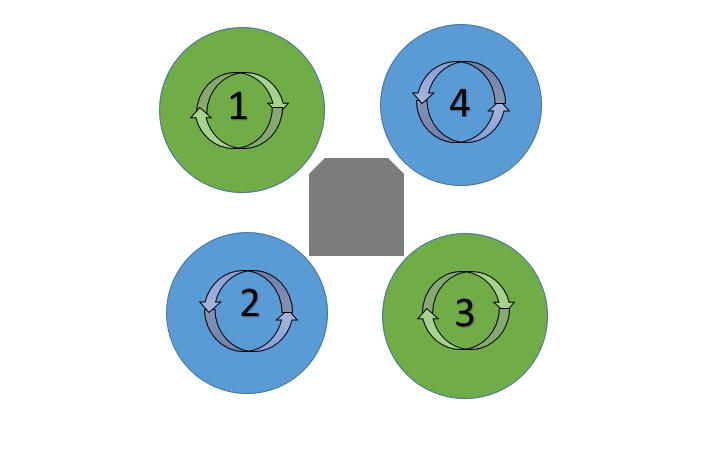
\includegraphics[width=0.44\columnwidth]{cross}%
	}
	\quad
	\subfloat[Общий вид \textit{plus}-схемы]{%
		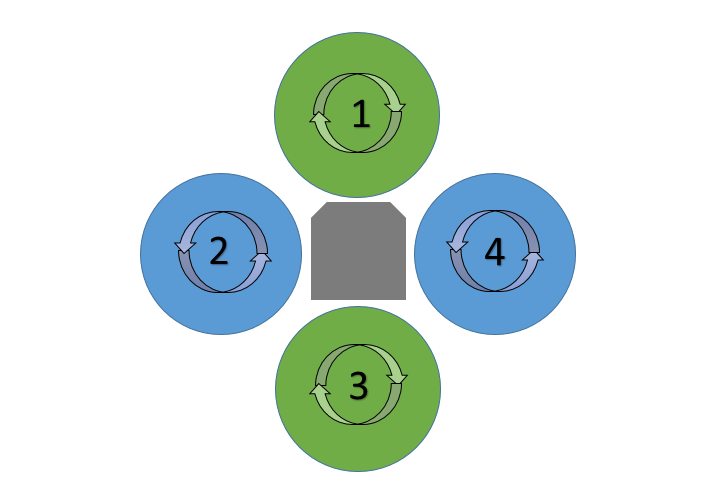
\includegraphics[width=0.44\columnwidth]{plus}%
	}
	\caption{ -- Основные схемы квадрокоптеров}
	\label{fig:cross_plus}
\end{figure}
Пропеллеры, расположенные на смежных лучах вращаются в разные стороны, благодаря чему возможна стабилизация по углу рысканья, при этом тяга каждого двигателя направленна одинаково. Вертикальное движение аппарата обусловлено изменением общей тяги всех двигателей. Горизонтальное движение совершается за счет изменения направления вектора тяги вследствие наклона корпуса БЛА \cite{Salih01}. 

\section{Основные подходы к построению модели динамики квадрокоптера}
	
Обычно, поступательное движение малых беспилотных летательных аппаратов рассматривают в инерциальной системе координат (назовем её {$I$}), связанной с поверхностью Земли. С учетом относительно небольших характерных расстояний и времен полета БЛА движением и кривизной поверхности Земли принебрегают.

Существуют два наиболее распространенных способа связать координатные оси с Землей: {$NED$} --  ось \textbf{$X_I$} направлена на север, ось \textbf{$Y_I$} -- на восток, а ось \textbf{$Z_I$} -- к центру Земли; {$ENU$} -- ось \textbf{$X_I$} направлена на восток, ось \textbf{$Y_I$} -- на север, а ось \textbf{$Z_I$} -- от центра Земли. Положение БЛА описывается радиус-вектором центра масс аппарата \bm{$r_I$},записанном в выбранной инерциальной системе координат. Скорость определяется, как
\begin{equation} \label{eq:velocity}
\bm{v_I} = \dot{\bm{r}}.
\end{equation}

Корпус квадрокоптера в рамках задачи управления движением обычно считают твердым телом. Для описания ориентации объекта в пространстве используют связанную с телом систему координат $B$, начало которой совпадает с центром масс БЛА, а оси направлены по главным центральным осям инерции корпуса (см. рис. \ref{fig:quad_scheme}). Текущее положение базиса B относительно I может быть описано матрицей поворота $\bm{R}_{IB}$, в том смысле, что разложения произвольного вектора $\bm{x}$, записанного в этих базисах, связаны соотношением
\begin{figure}[h!]
	\centering
	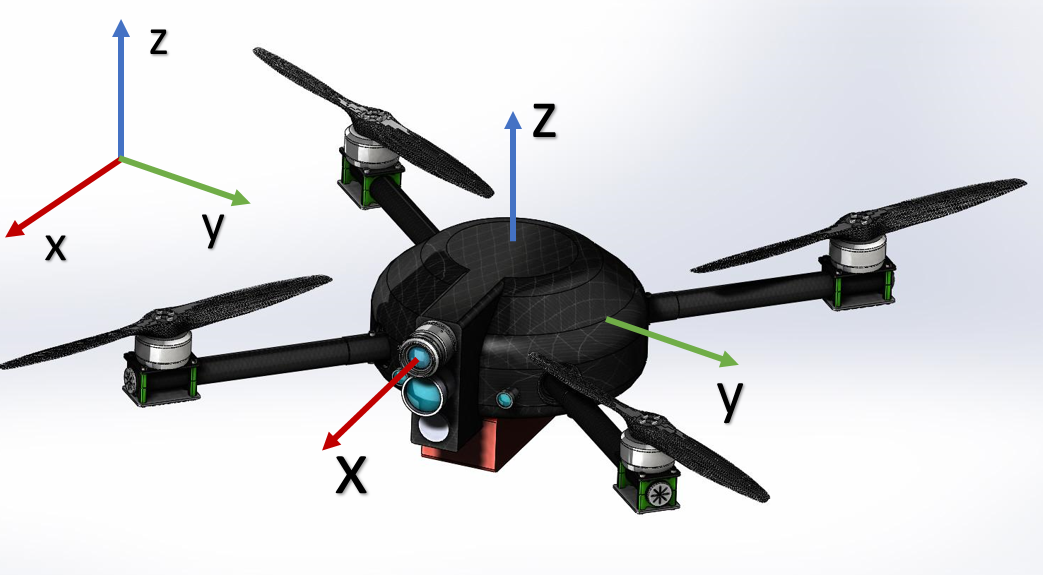
\includegraphics[width=0.9\columnwidth]{uavXYZ}
	\caption{ -- Квадрокоптер и системы кординат}
	\label{fig:quad_scheme}
\end{figure}
\begin{equation} \label{eq:rotmx}
\bm{x}_I = \bm{R}_{IB}\bm{x}_B.
\end{equation}
Матрица поворота связана с компонентами угловой $\bm{\Omega}_B$ скорости следующим соотношением
\begin{equation} \label{eq:angvel_rotmx}
\dot{\bm{R}}_{IB} = \bm{R}_{IB} [\bm{\Omega}_B]_{\times},
\end{equation}
где
\begin{equation} \label{eq:hat_operator}
[\bm{\Omega}]_{\times} =
\begin{bmatrix}
0            & -\bm{\Omega}^z   & \bm{\Omega}^y \\
\bm{\Omega}^z     & 0           &-\bm{\Omega}^x\\
-\bm{\Omega}^y    & \bm{\Omega}^x    & 0
\end{bmatrix}.
\end{equation}

Иногда для описания ориентации БЛА используют углы конечного поворота (иногда их называют углами Эйлера вне зависимости от последовательности), которые задают положение базиса B относительно базиса I через три  последовательных поворота вокруг осей связанной системы координат. Наиболее часто используются так называемые самолетные углы: последовательные повороты вокруг оси $Z_B$ на угол $\psi$, $Y_B$ на угол $\theta$, $X_B$ на угол $\phi$ будут определять углы рысканья, крена и тангажа. Им соответствует матрица поворота

\small
\begin{equation*} \label{eq:eul_to_rotmx}
\begin{aligned}
\bm{R} =
&\begin{bmatrix}
c(\psi)c(\theta) & c(\psi)s(\theta)s(\phi) - s(\psi)c(\phi) & c(\psi)s(\theta)c(\phi) + s(\psi)s(\phi) \\
s(\psi)c(\theta) & s(\psi)s(\theta)s(\phi) - c(\psi)c(\phi) & s(\psi)s(\theta)c(\phi) - c(\psi)s(\phi) \\
-s(\theta)         & c(\psi)s(\phi)                                 & c(\psi)c(\phi)\\
\end{bmatrix},
\end{aligned}
\end{equation*}
\normalsize
где для произвольного аргумента $x$ обозначим $c(x) = cos(x)$, $s(x) = sin(x)$. Обратное преобразование:
\begin{equation} \label{eq:rotmx_to_eul}
\begin{aligned}
&\psi  = \arctan\left( { - \frac{{{{\bm{R}}_{13}}}}{{{{\bm{R}}_{23}}}}} \right),
\\
\vspace{3mm}
\\
&{\theta  = \arccos  {{{\bm{R}}_{33}}} }
\\
\vspace{3mm}
\\
&\varphi  = \arctan\left( {\frac{{{{\bm{R}}_{31}}}}{{{{\bm{R}}_{32}}}}} \right)
\end{aligned}
\end{equation}

Помимо матриц и углов конечного поворота для описания ориентации часто используются кватернионы \cite{Amelkin01} -- четырехмерные гиперкомплексные числа, которые можно представить в виде формальной суммы скалярной и векторной частей
\begin{equation} \label{eq:quat_def}
Q = q_0 + \bm{q}.
\end{equation}
Для кватернионов определены операции сопряжения
\begin{equation} \label{eq:quat_dual}
\tilde{Q} = q_0 - \bm{q}
\end{equation}
и умножения
\begin{equation} \label{eq:quat_mult}
Q \circ P = q_0 p_0 - (\bm{q} \cdot \bm{p})
+ q_0 \bm{p} + p_0 \bm{q} + \bm{q} \times \bm{p}
\end{equation}
Кватернион ориентации  $q_{IB}$ определяет положение собственного базиса $B$ относительно базиса $I$ в том смысле, что разложения произвольного вектора $\bm{x}$, записанного в этих базисах, связаны соотношением
\begin{equation} \label{eq:quat}
\bm{x}_I = q_{IB} \circ \bm{x}_B \circ \tilde{q}_{IB}.
\end{equation}
Угловая скорость и кватернион ориентации связаны уравнением Пуассона
\begin{equation} \label{eq:puasson}
\dot{q}_{IB} = \frac{1}{2} {q}_{IB} \circ \bm{\Omega}_B.
\end{equation}
Кватернион ориентации эквивалентен матрице поворота
\begin{equation} \label{eq:quat_to_rotmx}
\bm{R} = ({q_0}^2 - \bm{q}^T \bm{q}) E_{3 \times 3} + 2 \bm{q}^T \bm{q} - 2 {q_0} [\bm{q}]_{\times},
\end{equation}
где $E_{n \times n}$ -- едичная матрица размерности $n$.
Его компоненты могут быть получены из углов Эйлера
\begin{equation}
\begin{aligned}
&{q_0} = \cos \frac{\theta }{2}\cos \frac{{\varphi  + \psi }}{2},
\\
\vspace{3mm}
\\
&{q_1} = \sin\frac{\theta }{2}\cos \frac{{\varphi  - \psi }}{2},
\\
\vspace{3mm}
\\
&{q_2} =  - \sin \frac{\theta }{2}\sin\frac{{\varphi  - \psi }}{2},
\\
\vspace{3mm}
\\
&{q_3} = \cos \frac{\theta }{2}\sin \frac{{\varphi  + \psi }}{2}.
\end{aligned}
\end{equation}

Движение центра масс БЛА определяется силами гравитации, аэродинамического сопротивления и тягой пропеллеров.
Иногда в моделях могут присутствовать и другие возмущения, например, учитывающие динамику полезной нагрузки \cite{Lim01}.
В их отсутствии уравнения для движения центра масс БЛА имеют вид
\begin{equation} \label{eq:common_traslational_motion}
m \ddot{\bm{r}} = \bm{F}_g + \bm{F}_{aero} + \bm{F}_{thr}.
\end{equation}
Основными параметрами, определяющими движение центра масс БЛА являются общая масса {$m$} конструкции, ускорение свободного падения \bm{$g$}, плотность среды {$\rho_{air}$}, аэродинамические свойства корпуса аппарата и пропеллеров. Сила тяжести определяется выражением

\begin{equation} \label{eq:gravity_force}
\bm{F}_g = m\bm{g}.
\end{equation}

Аэродинамические свойства корпуса БЛА определются площадью лобового сечения корпуса аппарата {$S_{\perp}$} и аэродинамическими константами. Выражение для аэродинамической силы можно записать, как \cite{Biard01}

\begin{equation} \label{eq:aerodynamic_force}
\bm{F}_{aero} = - \frac{1}{2} \rho_{air} C S_{\perp} |\dot{\bm{r}}| \dot{\bm{r}}.
\end{equation}

Такая модель позволяет учитывать ветер \cite{Bannwarth01}.
Силу тяги пропеллеров обычно определяют через квадрат их оборотов $\tilde\omega$ и аэродинамический коэффициент $k$ \cite{Falconi01}

\begin{equation} \label{eq:thrust_force}
\bm{F}_{thr} = \sum_{i=1}^{4}{ { k \tilde\omega^2_i \bm{z}_i}.}
\end{equation}
Здесь $\bm{z}_i$ -- ось вращения $i$-того пропеллера.
 
Вращательное движение корпуса БЛА определяется моментами сил, которые создают двигатели с пропеллерами и гироскопическим моментом самого корпуса

\begin{equation} \label{eq:common_rotational_motion}
\sum_{i=1}^{4}{\bm{\tau}_{Bi}} = \bm{J}_B\dot{\bm{\Omega}}_B + \bm{\Omega}_B \times  \bm{J}_B{\bm{\Omega}_B},
\end{equation}
где $\bm{J}_B$ -- тензор инерции корпуса БЛА, записанный в его главных осях.
Внешний момент, действующий на пропеллер, связывают с квадратом его оборотов с помощью аэродинамического коэффициента $b$ \cite{Ryll01}

\begin{equation} \label{eq:rotor_ext_torque}
\bm{\tau}_{Bi} = -b \tilde{\omega}^2_i \bm{z_i}.
\end{equation}
Также модель может включать в себя аэродинамические моменты \cite{Solovev01}.

При синтезе контура управления квадрокоптера стандартной конструкции в качестве компонентов вектора управления выбирают обороты его двигателей или некоторые их функции \cite{Sharifi01, Luukkonen01, Bemporad01}.  С учетом выражений (\ref{eq:thrust_force}), (\ref{eq:rotor_ext_torque}) удобно сформировать вектор управляющих воздействий из квадратов скоростей вращения пропеллеров

\begin{equation} \label{eq:common_control_vector}
u_i = \tilde{w}_i^2.
\end{equation}
Конкретные выражения для компонент зависят от рассматриваемой схемы квадрокоптера и способа нумерации его двигателей.
 
\section{Различные варианты постановки задачи управления}
Цели управления БЛА могут быть сформулированы по-разному,
начиная от приведения его центра масс в некоторое наперед заданное статичное положение
\cite{Huynh01, Yuskin01}
или обеспечения требуемой ориентации и высоты
\cite{Domingos01, Wang01, Gheorghita01, Lukmana01, Zabko01},
и заканчивая наблюдением за внешними объектами
\cite{Rodriguez01, Kendall01, Razinkova01}
и построением пространственных формаций
\cite{Ali01, Zhao01, Preiss01}.
 
Увеличение размерности вектора управляющего воздействия, например, за счет изменения угла атаки лопастей пропеллера \cite{Cutler01, Cutler02}  или изменения ориентации двигателей относительно корпуса \cite{Sridhar02, Kumar02} позволяет расширить маневренные возможности БЛА и усложнить поставленные перед ними задачи. Например, в работе \cite{Ryll02} в качестве задачи управления выбрано отслеживание аппаратом произвольной траетории в пространстве при независимом управлении ориентацией его корпуса. Подобная задача решена в исследовании \cite{Kaufman01} для БЛА с шестью двигателями с использованием пропеллеров с переменной геометрией. Применение таких пропеллеров для экстремальных маневров, включая фигуры высшего пилотажа, показали в работе \cite{Cutler02}.
 
Далее мы детально рассмотрим те техники и подходы, которые применяются для решения поставленных задач управления. 

\section{Управление с использованием ПИД-регуляторов}

ПИД-регуляторы широко используются в системах управления БЛА.
Такая популярность связана с их простой и понятной реализацией, а также рядом важных особенностей, таких, как способность устранять статические ошибки благодаря интегральной составляющей и прогнозировать состояние управляемой системы с помощью дифференциальной составляющей  \cite{Astrom01}.
Помимо этого, алгоритмы управления, использующие ПИД-регуляторы обычно не требуют больших вычислительных ресурсов.
Однако, существует ряд проблем при применении этой техники к построению систем управления квадрокоптероми, включающие нелинейности, связанные с математической моделью и неточностями моделирования динамики.
Поэтому применение ПИД-регуляторов для квадрокоптеров может ограничить их производительность \cite{Zulu01}.

Работа ПИД-регулятора основана на вычислении текущей ошибки положения в координатном пространстве $\bm{e}$, которая является разностью целевого состояния и оценки текущего состояния. Затем, управляющее воздействие вычисляется, как
\begin{equation} \label{eq:pid_common}
\bm{u}(t) = K_P \bm{e}(t) + K_I\int_0^t \bm{e}(t) dt + K_D \frac{d\bm{e}(t)}{dt},
\end{equation}
где $K_P$, $K_I$ и $K_D$ -- пропорциональный, интегральный и дифференциальный коэффициенты соответственно.

В работе \cite{Li01} применена схема с использованием ПИД-регулятора для управления положением и ориентацией БЛА.
Рассматриваемый аппарат спроектирован по \textit{plus}-схеме.
Ориентация аппарата описана углами Эйлера.
Динамическая модель включает в себя все основные силы и моменты (\ref{eq:common_traslational_motion}) - (\ref{eq:rotor_ext_torque}), действующие на аппарат, без каких-либо дополнительных возмущений.
Вектор состояния включает в себя скорость центра масс БЛА, углы его ориентации и их производные по времени.
Компоненты вектора управления являются функциями от квадратов скоростей вращения пропеллеров; первая компонента отвечает за общую тягу всех двигателей, остальные три -- за моменты сил, действующие вдоль собственных координатных осей.
Используя метод малых возмущений, авторы линеаризуют модель в окрестности текущего положения, находят передаточные функции по всем каналам управления, которые затем используют для построения \textit{Simulink}-модели.
Параметры модели соответствуют небольшому летательному аппарату с массой чуть больше одного килограмма.
В работе подобраны коэффициенты ПИД-регулятора, при которых БЛА удается стабилизировать свою позицию и ориентацию около целевой точки.
Далее в работе описан прототип летательного аппарата, реализующий предложенные алгоритмы.
Проведены летные испытания, ошибка по углам ориентации не превысила пяти градусов.

Последовательное применение ПД-регуляторов для управления положением и ориентацией используется в работе \cite{Mellinger01}. Рассматриваемый апарат также спроектирован по \textit{plus}-схеме.
Ориентация описывается углами Эйлера и с помощью матриц поворота.
Приведены некоторые аргументы в пользу использования простой модели двигателей
(\ref{eq:thrust_force}, \ref{eq:rotor_ext_torque}).
Компоненты вектора управляющего воздействия отвечают за тягу и моменты, действующие на корпус БЛА со стороны приводов:
\begin{equation} \label{eq:mellinger_control_vector}
	\begin{aligned}
	\bm{u} =
	\begin{bmatrix}
	k & k & k & k\\
	0 & bL & 0 & -bL\\
	-bL & 0 & bL & 0\\
	b & -b & b & -b
	\end{bmatrix}
	\begin{bmatrix}
	\omega^{2}_{1}\\
	\omega^{2}_{2}\\
	\omega^{2}_{3}\\
	\omega^{2}_{4}
	\end{bmatrix},
	\end{aligned}
\end{equation}
где $L$ -- расстояние от центра масс БЛА до осей вращения роторов.
Вектор состояния включает в себя позицию, ориентацию, а также линейную и угловую скорости аппарата
\begin{equation} \label{eq:mellinger_state}
\bm{x} = [\bm{r}_I, \phi, \theta, \psi, \bm{v}_I, \bm{\Omega}_B].
\end{equation}

Целью управления является отслеживание аппаратом траектории в пространстве и заданного угла рысканья. Авторы показывают, что модель является дифференциально плоской \cite{Belinskaya01, Nieuwstadt01} относительно выхода
\begin{equation} \label{eq:mellinger_flat_output}
\bm{\sigma} = (\bm{r},\psi)^T,
\end{equation}
то есть вектор состояния (\ref{eq:mellinger_state}) и вектор управляющих воздействий (\ref{eq:mellinger_control_vector}) может быть записан, как функция выхода  (\ref{eq:mellinger_flat_output}) и конечного числа его производных. Данный факт позволяет в дальнейшем строить оптимальные траектории в пространстве вектора выхода.

Синтезирован двухуровненвый контур управления. На первом уровне вычисляется ошибка позиционирования БЛА и используется ПД-регулятор для определения вектора целевой тяги квадрокоптера:
\begin{equation} \label{eq:mellinger_pos_err}
\bm{e}_r = \bm{r}^{0} - \bm{r},
\end{equation}
\begin{equation} \label{eq:mellinger_vel_err}
\bm{e}_v = \bm{v}^{0} - \bm{v},
\end{equation}
\begin{equation} \label{eq:mellinger_pos_reg}
\bm{F}^0 = K_r \bm{e}_r + K_v \bm{e}_v + m \bm{g} + m \ddot{\bm{r}}^0,
\end{equation}
где $\bm{r}^{0}$, $\bm{v}^{0}$, $\ddot{\bm{r}}^{0}$, $\bm{F}^{0}$ -- целевые координата, скорость, ускорение и общая сила тяги аппарата, а $K_r$ и $K_v$ -- некоторые положительно определенные матрицы.
Затем, положив $ || \bm{F}^{0} || > 0$
(что равносильно запрету на свободное падение БЛА),
авторы вычисляют первую компоненту вектора управляющих воздействий (\ref{eq:mellinger_control_vector}),
как
\begin{equation} \label{eq:mellinger_u1}
u_1 = \bm{F}^{0} \cdot \bm{z}_B,
\end{equation}
и определяют целевую ориентацию при известном угле рысканья из условия
\begin{equation} \label{eq:mellinger_Rdes}
\bm{R}_{IB}^0 [0,0,1]^T = \frac{\bm{F}^{0}}{||\bm{F}^{0}||}.
\end{equation}
На основе ошибки ориентации
\begin{equation} \label{eq:mellinger_eR}
\bm{e}_R = \frac{1}{2}
\Big[
(\bm{R}_{IB}^0)^T 	\bm{R}_{IB} -
(\bm{R}_{IB})^T \bm{R}_{IB}^0
\Big]_\vee,
\end{equation}
где оператор $[...]_\vee$ является обратным преобразованием к (\ref{eq:hat_operator}), и ошибки по угловой скорости вычисляются оставшиеся компоненты вектора управляющих воздействий
\begin{equation} \label{eq:mellinger_att_reg}
[u_2, u_3, u_4]^T = K_R \bm{e}_R + K_{\Omega} \bm{e}_{\Omega}.
\end{equation}
Затем, авторы вычисляют значения оборотов каждого из двигателей на основе выражения (\ref{eq:mellinger_control_vector}).
	
В заключительной части работы рассматривается вопрос построения траекторий. Авторы строят кусочно-полиминиальную кривую через набор точек маршрута, минимизируя интеграл квадрата нормы второй производной ускорения центра масс аппарата и интеграл квадрата нормы второй производной угла его рысканья. Затем  авторы показывают, как можно локализовать некоторые участки траектории в прямоугольной области, для того, чтобы избежать их пересечений с возможными препятствиями.

Производительность алгоритмов демонстрируется в натурном эксперименте. Траекторией БЛА является окружность, скорость аппарата превышает два с половиной метра в секунду, а углы крена тангажа достигают сорока градусов. Ошибка позиционирования не превышает пятнадцати сантиметров, однако ошибка ориентации авторами не приводится. Важной особенностью работы является учет нелинейной природы динамики квадрокоптера при синтезе контура управления. Это позволяет сохранять устойчивость управления при значительных отклонениях корпуса аппарата по углам тангажа и рысканья.

Исследование относительной эффективности применения ПИД регулятора для стабилизации ориентации корпуса квадрокоптера проводят авторы работы \cite{Bouabdallah01}. Кроме стандартных возущений, в модели присутствуют выражения для динамики бесколлекторных двигателей. Для синтеза контура управления авторы принебрегают гироскопическими эффектами со стороны двигателей с пропеллерами, упрощают и линеаризуют модель в окрестности точки соотвествующей неподвижному зависанию БЛА в воздухе. Ошибка ориентации, равная разнице целевого и текущего положения, записанных в углах Эйлера, подается на вход ПИД-регулятора, затем вычисляется вектор управления. Проведены вычислительные эксперименты и эксперименты на тестовом стенде. Авторы отмечают хорошую производительность алгоритмов управления, принимают во внимание эффекты, возникающие из-за более подробного моделирования динамики роторов и отмечают необходимость быстрого реагирования приводов робота на управление.

Затем происходит синтез второго контура управления, в основе которого лежит линейно-квадратичный регулятор (ЛК-регулятор, ЛКР) и сравнение полученных результатов.
	

\section{Управление с использованием ЛК-регуляторов}

Линейно-квадратичный регулятор -- один из видов оптимальных регуляторов, который применяется в линейных системах вида
\begin{equation} \label{eq:linear_dyn_system}
\dot{\bm{x}} = A\bm{x} + B\bm{u}
\end{equation}
и  использует квадратичный функционал вида
	\begin{equation} \label{eq:lqr_cost_func}
	F = \int_0^{\infty}{(\bm{x}^T Q \bm{x} + \bm{u}^T R \bm{u})} dt
	\end{equation}
в качестве критерия оптимальности. Управление, минимизируещее функционал \eqref{eq:lqr_cost_func}, имеет вид \cite{Letov01}
	\begin{equation} \label{eq:lqr_control_law}
	\bm{u} = -R^{-1} B^T P \bm{x},
	\end{equation}
где $P$ находится из решения уравнения Риккати
	\begin{equation} \label{eq:riqatty}
	A^T P + P A - P B R^{-1} B^T P + Q = -\dot{P}.
	\end{equation}
Такой подход относительно распространен при проектировании систем управления роботов, в том числе и мультикоптеров \cite{Baklanov01, Muhhamid01, Argentim01} и позволяет оптимизировать некоторые параметры движения. Однако, как отмечают авторы некоторых работ, производительность ЛК-регуляторов сильно зависит от полноты математической модели и точности определения параметров динамики системы \cite{Kim01, Joukhadar01}. Рассмотрим некоторые работы более подробно.

Сравнение эффективности различных подходов для синтеза системы управления квадрокоптером приведено в работе \cite{Bouabdallah01}. Для того чтобы применить линейно-квадратичного регулятор, авторы линеаризуют модель в окрестности текущего положения, затем решают уравнение Рикатти и находят компоненты вектора управляющего воздействия.
Численные и стендовые эксперименты показывают, что такой подход обеспечивает лучшую стабилизацию аппарата в пространстве, чем при применении ПИД-регулятора, что может быть следствием использования более полной модели динамики БЛА при синтезе ЛК-регулятора.

Подобным образом проектируют систему управления квадрокоптером авторы работы \cite{Reyes-Valeria01}. Модель аппарата исполнена по \textit{plus}-схеме. Кинематика вращательного движения представлена в кватернионном описании. Вектор состояния содержит положение центра масс аппарата, его скорость, кватернион ориентации и угловую скорость. Динамика аппарата, помимо стандартных сил и моментов, содержит аэродинамические моменты, действующие на корпус БЛА. Для линеаризации модели авторы выбирают точку неподвижного зависания квадрокоптера и затем строят ЛК-регулятор, который определяет оптимальную траекторию в его координатном пространстве. Из-за нестабильного поведения системы вдали от целевой траектории авторы синтезируют второй, независимый регулятор, который заменяет первый в случае значительных отклонений от целевых параметров движения. Работоспособность контура управления иллюстрируется численными экспериментами. Графики демонстрируют сходимость траектории к целевой, при этом углы ориентации в процессе движения не приводятся.

Оригинальный подход к решению проблемы большой чуствительности систем управления на основе ЛК-регулирования к точности модели и текущих параметров движения показан в работе \cite{Minh01}. Авторы расширяют модель системы \eqref{eq:linear_dyn_system}, добавив возмущения $G \bm{w}$ и шум измерений $\bm{v}$
\begin{equation} \label{eq:linear_dyn_system_noisy}
\begin{aligned}
&\dot{\bm{x}} = A\bm{x} + B\bm{u} + G \bm{w}\\
&\bm{y} = C \bm{x} + \bm{v}.
\end{aligned}
\end{equation}
Затем для оценки состояния используется расширенный фильтр Калмана и применяется линейно-квадратичное гауссовское (ЛКГ) управление с интегральным действием. Численные эксперименты демонстрируют возможность стабилизировать аппарат в некоторой точке. Преимущество ЛКГ подхода заключается в отсутствии необходимости очень точно оценивать текущее состояние объекта управления. К сожалению, авторы не показали производительность алгоритмов управления для более сложных маневров.

%% SLIDE MODE
\section{Управление с использованием скользящего режима}

Скользящий режим (\textit{sliding mode}) -- один из видов робастного управления, при котором управляющие воздейтвие на объект обеспечивает его движение в пределах выбранной поверхности в фазовом пространстве, не позволяя выбранным параметрам выходить за пределы допустимых, чем обеспечивается устойчивость такого движения.
При смещении траектории объекта за пределы поверхности включается активное управление, кторое возвращает его на одну из допустимых траекторий.
К преимуществам этого подхода можно отнести отсутствие необходимости линеаризовывать уравнения движения и малая чуствительность к изменениям параметров динамики управляемого объекта, что весьма актуально для синтеза систем управления мультироторными роботами.
Однако, использование такого подхода требует особой осторожности, так как неучтенные эффекты в работе исполнительных органов системы управления могут привести к вибрациям, потере энергии и другим нежелательным эффектам \cite{Utkin01}.

Синтез системы управления с использованием метода скользящего режима включает в себя два основных шага. На первом шаге необходимо выбрать поверхность в фазовом пространстве, движение в окрестности которой обеспечит сходимость состояния системы к целевому. Для системы
\begin{equation} \label{eq:slide_mode_system}
\dot{\bm x} = f(\bm x, t) + g( \bm x, t) \bm u,
\end{equation}
где $\bm x$ -- вектор состояния, $\bm u$ -- вектор управляющих воздействий, в качестве такой поверхности обычно выбирают \cite{Samir01}
\begin{equation} \label{eq:slide_mode_S}
S(\bm x) = \bm e + \lambda \dot{\bm e},
\end{equation}
где $\bm e$ -- рассогласование текущего и целевого состояния, $\lambda > 0$ -- некоторая константа. На втором шаге происходит поиск закона управления, который приводит и сохраняет траекторию системы в окрестности заданной на предыдущем шаге поверхности.
\begin{equation} \label{eq:slide_mode_on_S}
S(\bm x,t) = 0.
\end{equation}
Такой подход применяется как для квадрокоптеров \cite{Stevanovic01, Lebedev01, Xu01}, так и для летающих роботов другой конструкции \cite{Yih01, Zhu01}. Рассмотрим некоторые примеры.

В работе \cite{Samir01} скользящий режим применяется для синтеза управления квадрокоптера \textit{cross}-конфигурации.
Модель (\ref{eq:common_traslational_motion}, \ref{eq:common_rotational_motion}, \ref{eq:rotor_ext_torque}, \ref{eq:thrust_force}) дополнена динамикой бесколлекторных двигателей.
Авторы синтезируют двухуровневый контур управления, последовательно применяя скользящий режим для положения и ориентации объекта. При этом сначала, используя величину общей тяги квадрокоптера, стабилизируется высота аппарата, а затем второй регулятор обеспечивает необходимые для заданного горизонтального движения углы крена и тангажа. Численные эксперименты показали способность предложенных алгоритмов стабилизировать аппарат в точке, удаленной от исходной на расстоянии чуть более 3 метров за время около 10 секунд.

Скользящий режим также используется в работе \cite{Runcharoon01}. Здесь, подобно \cite{Samir01}, синтезируется двухуровневый контур управления, однако \textit{sliding mode} регулятор отвечает только за ориентацию корпуса БЛА, когда как ПД-регулятор -- за его позицию. Выражения для компонент вектора управляющего воздействия авторы определяют, полагаясь на результаты \cite{Slotine01}. Основным отличием, при этом, является использование более «гладкого» управления в окрестности целевой поверхности $S(\bm x)$. Вычислительные эксперименты демонстрируют, что данный шаг значительно сокращает время сходимости  ориентации корпуса БЛА к целевой. 

Отдельное внимание стоит уделить исследованию \cite{Sumantri01}, где использовалась нелинейная поверхность $S(\bm x)$, что позволило значительно повысить устойчивость БЛА к внешним возмущениям.

%% Robust Control
\section{Робастное управление}

В реальных задачах часто бывает невозможно с абсолютной точностью определить модель рассматриваемого объекта или параметры его динамики.
В случае необходимости гарантировать качество управления и оценить влияние таких неточностей на движение управляемого объекта используют обширный функционал теории робастного управления.
При описании системы с помощью передаточных функций неопределенный объект можно описать как
\begin{equation} \label{eq:robust_ctrl_obj}
H(s, q) = \frac{A(s, q)}{B(s, q)}, q \in Q,
\end{equation}
где $A(s, q)$ и $B(s, q)$ -- неопределенные полиномы, коэффициенты которых зависят от $q \in Q$ \cite{Polyak01}. 

Такой подход может оказаться весьма полезен при рассмотрении управляемой динамики
мультироторных летающих роботов, параметры которой могут изменяться в известных пределах, в том числе из-за использования разной полезной нагрузки или постепенного износа пропеллеров. Среди примеров использования теории робастного управления для проектирования систем управления БЛА можно отметить работы \cite{Lee02, Borisov01, Petranevsky01, Bai01, Tony01}. Рассмотрим содержание последней.

После некоторых упрощений, авторы формулируют модель динамики квадрокоптера как 
\begin{equation} \label{eq:Tony_dyn}
\ddot{\bm x} = f(\bm x) + g( \bm x) \bm u + d(t),
\end{equation}
где вектор состояния $\bm x$ составлен из высоты и ориентации аппарата, представленной углами Эйлера, а возмущение $d(t)$ является неизвестной нелинейной и гладкой функцией времени. Цель управления -- асимптотическая сходимость центра масс БЛА к целевой траектории. Для выполнения поставленной задачи авторы вынуждены работать с рядом начальных предположений, например, модуль возмущения $d(t)$, а также первой и второй его производной ограничены некоторыми известными значениями. Подобные ограничения также сформулированы для параметрически заданой целевой траектории $\bm x_d(t)$ и других параметров модели. В результате исследователям удается синтезировать контур управления, работоспособность которого подтверждена численными экспериментами, где БЛА стабилизируется в окрестности заданной точки, при этом авторы отмечают, что возмущения при этом соответствуют относительной ошибке измерения массы от 20\% до 50\%.

%% Feedback Linearization
\section{Метод линеаризации обратной связью}

Метод линеаризации обратной связью применяют для нелинейных систем вида
\begin{equation} \label{eq:feedback_linearization_system}
\begin{aligned}
&\dot{\bm x} = f(\bm x) + g(\bm x) \bm u\\
&\bm y = h(\bm x),
\end{aligned}
\end{equation}
где $\bm x$ -- вектор состояния, $\bm u$ -- вход системы, $\bm y$ -- ее выход.
Суть метода состоит в поиске преобразования 
\begin{equation} \label{eq:feedback_linearization_transform}
\bm z = T(\bm x),
\end{equation}
и закона управления вида
\begin{equation} \label{eq:feedback_linearization_control}
\bm u = \alpha(\bm x) + \beta(\bm x) \bm v,
\end{equation}
где $\bm v$ -- новый вход системы , которые преобразуют нелинейную систему \eqref{eq:feedback_linearization_system} в эквивалентную линейную \cite{Slotine01}. Метод достаточно широко используется как для управления отдельными мультироторными роботами \cite{Chang01, Freddi01}, так и в области группового управления БЛА \cite{Mahmood01}. Рассмотрим некоторые примеры подробнее.

Воспользоваться методом линеаризации обратной связью для синтеза системы управления квадрокоптером удалось в работе \cite{Roza01}. Рассматривается квадрокоптер \textit{plus}-конфигурации. Авторы используют стандартную модель динамики БЛА такой конструкции (\ref{eq:common_traslational_motion}, \ref{eq:common_rotational_motion}, \ref{eq:rotor_ext_torque}, \ref{eq:thrust_force}), исключив силу аэродинамического сопротивления, при этом пояснив, что планируют добавить в модель это и другие возмущения в следующих работах. Постановка задачи требует асимптотической сходимости траектории центра масс БЛА к целевой, при которой функции его текущей скорости и угла рысканья также имеют асимптотическую сходимость к заданным значениям, которые, в свою очередь, зависят от смещения аппарата вдоль траектории. В вычислительном эксперименте в качестве траектории авторы выбрали плоскую окружность радиусом 10 метров и продемонстрировали принципиальную возможность выполнять летное задание на скоростях 3 м/с и 15 м/с, при этом величина отклонения от траектории в процессе движения не приводится.

В работе \cite{Kanatnikov} рассматривается упрощенная модель движения квадрокоптера, где отсутсвует сила аэродинамического сопротивления и некоторые другие, не очень значительные эффекты.
Затем по отдельности рассматривается движение БЛА в горизонтальной и вертикальной плоскости.
Показано, что двухкратное дифференцирование уравнений горизонтального движения квадрокоптера позволяет привести систему к каноническому виду 
\begin{equation*}
\begin{bmatrix}
&x\\ &y
\end{bmatrix} ^{IV}
=
P + Q \bm{u},
\end{equation*}
что позволяет синтезировать контур управления.

Исследование относительной эффективности метода линеаризации обратной связью приведено у \cite{Lee01}. Показано, что в сравнении с некоторыми другими подходами метод обладает большей чувствительностью к шуму измерений и неточностям модели. Авторы делают вывод, что синтез контура управления с использованием метода линеаризации обратной связью можно эффективно применять совместно с другими алгоритмами, чтобы уменьшить влияние возмущений различной природы.

%% 
\section{Адаптивное управление}

Адаптивное управление -- широкий класс алгоритмов, позволяющих проектировать систему управления способной изменять параметры или структуру регулятора в зависимости от изменения параметров управляемого объекта или внешних возмущений.
Применение подобных алгоритмов для БЛА может быть обусловлено изменчивостью параметров динамики во время полета, например вследствие значительного снижения заряда батареи или наличия аэродинамических возмущений вблизи горизонтальной поверхности. Помимо этого, как удтверждают некоторые авторы, применение алгоритмов адаптивного управления позволяет не учитывать некоторые параметры динамики мультикоптеров \cite{Belyavskiy01}. Стоит отметить наиболее заметные работы, где используются алгоритмы адаптивного управления применительно к БЛА: \cite{Dydek01, Mu01, Bara01}.

В исследовании \cite{Bara01} рассматривается квадрокоптер стандартной конструкции, выполненный по \textit{cross}-схеме. Ориентация представленна углами Эйлера. Синтезирован двухуровневый контур управления, на первом уровне применяется регулятор на основе скользящего режима для управления горизонтальным положением БЛА. На втором уровне используется адаптивный регулятор для управления выделенной из модели полностью управляемой подсистемой, вектор состояния которой составлен из ориентации и общей тяги БЛА. Рассмотрено два подхода к построению адаптивного управления -- первый использует ошибку текущего положения и ориентации для оценки параметров динамики объекта, второй дополнительно использует разницу между измеренным и оцененным выходами управления. Комбинированный подход показал хорошую производительность в условиях полной неопределенности для ключевых параметров динамической модели.

Применение адаптивного управления для стабилизации движения квадрокоптера со смещающимся во времени центром масс рассмотрено в исследовании \cite{Palunko01}. Авторы применили линеаризацию обратной связью с последующим применением ПД-регулятора и показали, что такое управление неспособно справиться со стабилизацией движения БЛА. Затем применен аддитивный адаптивный компонент системы управления, с помощью которого оценивалось смещение центра масс аппарата и происходила коррекция рассчета управляющего вектора.

%% BACKSTAPPING
\section{Управление с использованием метода декомпозиции}

Метод декомпозиции (\textit{backstapping}) -- рекурсивный алгоритм, основанный на разбиении динамической системы на набор подсистем и поочередной стабилизации каждой из них. Метод активно применяется для мультироторных роботов \cite{Pota01, Chen01, Jung01, Huo01}.

В работе \cite{Madani01} показано, что алгоритм не является вычислительно затратным и неплохо справляется с возмущениями, однако чувствителен к точности в оценках параметров модели. Основная идея применения метода декомпозиции в исследовании состоит в том, чтобы стабилизировать систему в два этапа. Сначала осуществляется управление горизонтальной позицией аппарата с помощью виртуального входа, использующего в качестве компонент некоторые функции от углов рысканья и тангажа. Затем, управление ориентацией осуществляется посредством изменения скорости роторов.

\section{Оптимальное управление}

Оптимальное управление основано на поиске регулятора, который обеспечит минимизацию целевого функционала, сформулированного с учетом контекста задачи.
Для БЛА целью оптимального управления может быть минимизация расхода энергии \cite{Morbidi01, Huang01}, максимизация длительности или дальности полета \cite{Cowling01, Suicmez01}, движение по наилучшей (по выбранному критерию) траектории в присутствии препятствий \cite{Chen02, Cheng01} и другие.
Обычно ситема управления в основе которой лежат принципы оптимального управления не отличается робастностью и для ее успешного синтеза требуется с большой точностью определить параметры системы.

Синтез $L_1$ оптимального регулятора, обладающего относительно неплохими робастными качествами описан в работе \cite{Satici01}. Авторам удалось минимизировать негативные эффекты, возникающие в из-за ошибки оценки текущего состояния и возмущений без их непосредственного измерения.

$H_{\infty}$ оптимальное управление применялось к упрощенной модели динамики квадрокоптера в исследовании \cite{Falkenberg01}. Алгоритм показал очень высокую производительность даже в условиях сильных возмущений.

Для управления ориентацией БЛА и отслеживания целевых траекторий в работе \cite{Raffo01} синтезирован интегральный $H_{\infty}$ оптимальный регулятор. Численные эксперименты показали хорошую сопротивляемость помехам и возмущениям. Интегральная составляющая имела важное значение для качества управления.

\section{Управление с использованием искуственных нейронных сетей и алгоритмов нечеткой логики}

Применение искуственных нейронных сетей и алгоритмов нечеткой логики (\textit{fuzzy logic}) в приложении к системам управления мультироторными роботами в последнее время стало популярным и продемонстрировало свою эффективность. Нечеткая логика  -- обобщение классической теории множеств и логики, в основе которого лежит понятие нечеткого множества, где функция принадлежности элемента к множеству не является бинарной.

Примером применения алгоритмов нечеткой логики является работы \cite{Dierks01} и \cite{Santos01}. Авторы интерпретируют текущую ошибку положения и ориентации БЛА как элемент нечеткого множества, затем синтезируется ПИД-регулятор. Численные эксперементы демонстрируют принципиальную возможность управления квадрокоптером с использованием этого подхода.

Искуственные нейроныые сети -- класс алгоритмов, основанный на подборе параметров (обучении) функции специального вида (нейросети) таким образом, чтобы эта функция вела себя желательным образом на рассматриваемой множестве. Таким образом, алгоритм можно применить для управления системами; в качестве входа может быть рассмотрена ошибка состояния, а в качестве выхода -- сигнал управления, который будет устранять эту ошибку. Подобным образом поступили в работе \cite{Nicol01}. Авторам удалось спроектировать систему таким образом, чтобы она была асимптотически устойчивой.

В работе \cite{Evgenov01} с помощью искуственной неройной сети создана система автоматического субоптимального подбора коэффициенов ПИД-регулятора, отвечающего за положение и ориентацию квадрокоптера, из-за чего система управления приобретает свойства адаптивной.

Методы глубокого обучения применялись в работе \cite{Andersson01}. Авторы обучили нейронную сеть с помощью самостоятельно созданного алгоритма, оптимизирующего траектории в координатном пространстве, смогли учесть неточности модели, ограничения на максимальную силу тяги роторов и наличие препятсвий.
Затем они показали пример успешного применения алгоритма при использовании небольших вычислительных ресурсов.

\section{Квадрокоптеры с расширенным вектором управляющего воздействия}

Для увеличения маневреных характеристик квадрокоптеров и повышения их общей управляемости многие исследователи придпринимали попытки усовершенствовать конструкцию БЛА. Одним из вариантов таких изменений является использование специальных приводов, способных изменять геометрию пропеллеров в полете, тем самым увеличивая некоторые характиристики БЛА.

Работа \cite{Cutler01} наглядно демонстрирует преимущества квадрокоптеров с изменяющейся геометрией воздушных винтов. Описана расширенная модель двигателей и пропеллеров, которая затем линеаризуется. Реализованы несколько вариантов управления. Эксперименты показывают снижение потребления энергии в полете а также способность БЛА усовершенствованной конструкции выполнять сложные маневры, недоступные стандартному квадрокоптеру, например, зависать в перевернутом положении. Продолжение исследования приведено в работе \cite{Cutler02}, где авторы принимают во внимание ограничения на выходы приводов БЛА и строят траектории с учетом этих ограничений.

Другой распространенный способ расширить размерность вектора управляющего воздействия БЛА -- добавить возможность изменять направления тяги его двигателей \cite{Papachristos01, Gupta01, Lin01, Dharmawan01}. Управляемой динамике таких аппаратов посвящено много работ, среди которых большая часть опубликована в последние годы.

Одну из реализаций контура управления для квадрокоптера с поворотными роторами предложили в статье \cite{Ryll01}. Исследователи рассматривают квадрокоптер \textit{cross}-схемы c двигателями, которые могут вращаться вокруг лучей, к которым они прикреплены (рис. \ref{fig:ryll_scheme}). Модель динамики аппарата рассматривает основные внешние силы и моменты, действующие на аппарат (\ref{eq:common_traslational_motion}, \ref{eq:thrust_force}, \ref{eq:common_rotational_motion}, \ref{eq:rotor_ext_torque}), а также подробно описывают взаимодействие каждого из поворотных роторов с корпусом. Для этого рассчитывается полная угловая скорость каждого ротора с пропеллером в проекциях на собственные оси
\begin{equation}
\bm{\omega}_{R_i} = ~^B\bm{R}_{R_i}^T \bm \Omega_B + [\dot{\theta}_i \ 0 \ \tilde \omega_i]^T,
\end{equation}
где $~^B\bm{R}_{R_i}^T$ -- матрица поворота, представляющая ориентацию $i$-того ротора с пропеллером
относительно корпуса аппарата.
Затем записываются динамические уравнения Эйлера, откуда может быть получен момент, действующий со стороны луча на поворотный ротор
\begin{equation}
\bm{\tau}_{R_i} = \bm J_{R_i} \dot{\bm \omega}_{R_i} +
{\bm \omega}_{R_i} \times \bm J_{R_i} {\bm \omega}_{R_i} - \bm \varsigma_i,
\end{equation}
где $\bm \varsigma_i$ -- внешний момент, действующий на пропеллер \eqref{eq:rotor_ext_torque}.

Цель управления -- обеспечение движения центра масс аппарата по целевой траектории при независимом управлении ориентацией корпуса. 
\begin{figure}[h!]
	\centering
	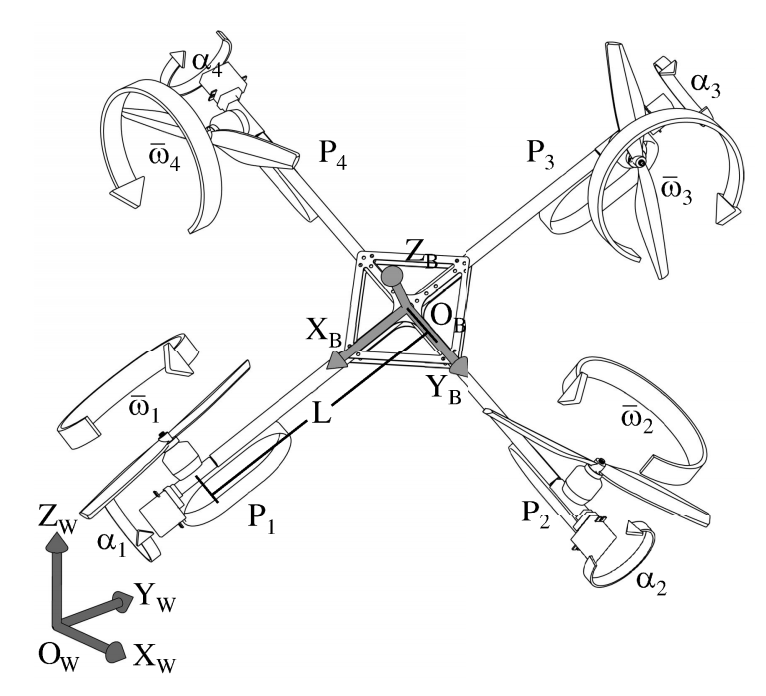
\includegraphics[width=0.65\columnwidth]{ryll_scheme}
	\caption{ -- Общая схема БЛА, расмматриваемого в работе \cite{Ryll01} (рисунок авторов)}
 	\label{fig:ryll_scheme}
\end{figure}
%%%!"!!!!!!!!!!!!!!!!!!!!!!!!!!!!!!!!!!!!

В вектор состояния входят координаты ценра масс аппарата и его ориентация, представленная в матричном виде.
В качестве компонент вектора управляющего воздействия выбраны скорости изменения оборотов двигателей с пропеллерами и скорости поворота двигателей вокруг соответсвующих лучей.
\begin{equation} \label{eq:ryll_ctrl_out}
\begin{aligned}
&\bm{u} = (\dot{\bm \omega}_u,  \dot{\bm \theta}_u)^T,
\\
\bm \omega_u =
(\tilde\omega_1 |\tilde\omega_1|,
\tilde\omega_2 |\tilde\omega_2|&,
\tilde\omega_3 |\tilde\omega_3|,
\tilde\omega_4 |\tilde\omega_4|)^T,
\quad
{\bm \theta}_u = (\theta_1, \theta_2 , \theta_3 , \theta_4 )^T.
\end{aligned}
\end{equation}

Для синтеза контура управления авторы упрощают динамическую модель, принебрегая некоторыми эффектами,
в том числе силой аэродинамического сопротивления, гироскопическими эффектами со стороны корпуса аппарата и роторов с пропеллерами. Преобразованная модель принимает вид
\begin{equation} \label{eq:ryll_dyn}
\begin{aligned}
&\ddot{\bm r}_I = \bm F_g + \frac{1}{m}~^I \bm R_B \bm F(\bm \theta_u) \bm \omega_u,
\\
&\dot {\bm \Omega}_B = \bm J_B \bm T(\bm \theta_u) \bm \omega_u,
\end{aligned}
\end{equation}
где матрицы $\bm F(\bm \theta_u)$ и $\bm T(\bm \theta_u)$ отвечают за текущую геометрию аппарата и с учетом выбранной схемы (рис.\ref{fig:ryll_scheme}) 
\begin{equation} \label{eq:ryl_dyn_matrixes}
\begin{aligned}
&\bm F(\bm \theta) =
\begin{bmatrix}
0&-ks_2&0&ks_4\\
-ks_1&0&ks_3&0\\
kc_1&-kc_2&kc_3&-kc_4
\end{bmatrix},
\\
\phantom{}
\\
&\bm T(\bm \theta) =
\begin{bmatrix}
0&-Lkc_2&0&Lkc_4\\
-Lkc_1&0&Lkc_3&0\\
-Lks_1&Lks_2&-Lks_3&Lks_4
\end{bmatrix}
+
\begin{bmatrix}
0&-bs_2&0&bs_4\\
bs_1&0&-bs_3&0\\
-bc_1&-bc_2&-bc_3&-bc_4
\end{bmatrix}, 
\end{aligned}
\end{equation}
где $c_i = \cos(\theta_i)$, $s_i = \sin(\theta_i)$.
Затем выражения \eqref{eq:ryll_dyn} дифференцируют по времени
\begin{equation} \label{eq:ryll_dyn_dot}
\begin{aligned}
\begin{bmatrix}
&\dddot{\bm r}_I
\\
&\ddot{\bm \Omega}_B
\end{bmatrix}
=
\bm A(\bm \theta_u, \dot {\bm \omega}_u)
\begin{bmatrix}
&\dot{\bm \omega}_u
\\
&\dot{\bm \theta}_u
\end{bmatrix}
+
\bm b(\bm \theta_u, \bm \omega_u, \bm \Omega_B).
\end{aligned}
\end{equation}
Для решения поставленной задачи управления авторы синтезирует регулятор,
\begin{equation} \label{eq:ryll_reg}
\begin{aligned}
\dddot{\bm{r}_d}(t)&=
\dddot{\bm{r}}^0(t) +
\bm{K}_{r1}(\ddot{\bm{r}}^0(t) - \ddot{\bm{r}}(t)) +
\bm{K}_{r2}(\dot{\bm{r}}^0(t) - \dot{\bm{r}}(t)) + 
\bm{K}_{r3}\delta \bm r,
\\
\ddot{\bm{\Omega}_d}(t)&=
\ddot{\bm{\Omega}}^0(t)
+ \bm{K}_{\Omega1}(\dot{\bm{\Omega}}^0(t)-\dot{\bm{\Omega}}(t))
+ \bm{K}_{\Omega2}(\bm{\Omega}^0(t)-\bm{\Omega}(t))
+ \bm{K}_{\Omega3}\delta\bm{R},
\end{aligned}
\end{equation}
сходимость которого обеспечивается выбором матриц коеффициентов $\bm K_{\times}$, которые должны удовлетворять критерию Рауса-Гурвица, а затем обращают динамику и находят вектор $\bm u$, используя псевдообращение Мура-Пенроуза \cite{Barata01}
\begin{equation} \label{eq:ryll_inversed}
\begin{aligned}
\begin{bmatrix}
&\dot{\bm \omega}_u
\\
&\dot{\bm \theta}_u
\end{bmatrix}
=
\bm A^+ \left(
\begin{bmatrix}
&\dddot{\bm r}_I
\\
&\ddot{\bm \Omega}_B
\end{bmatrix}
+
\bm b
\right)
+
(\bm E_8 - \bm A^+ \bm A) \bm \zeta.
\end{aligned}
\end{equation}

Вектор $\bm \zeta$ позволяет использовать две дополнительные степени свободы, возникающих в результате того, что размерность вектора управляющих воздействий превышает размерность вектора состояния, для поддержания ненулевых значений оборотов двигателей, что необходимо для возможности псевдообращения матрицы $\bm A$.

Авторы отмечают, что при реализации обратных связей в контуре управления возможны сложности
с оценкой второй производной текущего положения и ориентации, входящих в регулятор \eqref{eq:ryll_reg},
так как численное дифференцирование сигнала инерциальных датчиков приведет к высокому уровню шума.
Для оценки этих параметров движения предложно воспользоваться выражениями \eqref{eq:ryll_dyn_dot}.
При этом позиция, скорость, ориентация и угловая скорость
измеряется с помощью внешней следящей системы,
также на борту обеспечены измерения оборотов двигателей и углов отклонения сервоприводов.

Для уточнения параметров динамики модели авторы проводят ряд измерений, экспериментально уточняя аэродинамические свойства пропеллеров и переходные процессы в сервоприводах, отвечающих за наклон двигателей.

В работе приводятся численные эксперименты, а после исследователи демонстрируют воплощение алгоритмов управления в прототипе.
В качестве траектории показательного полета выбрана плоская "восьмерка".
Ошибка позиционирования БЛА составила около 5 сантиметров, ориентации -- не более 0,1 радиана.

Основным преимуществом этой работы является детальное рассмотрение управляемой динамики БЛА с поворотными роторами, подробное описание алгоритмов и способов инженерной реализации БЛА такой конструкции.
К недостаткам можно отнести необходимость оценки рывка и углового ускорения в каждый момент времени, а предложенный способ такой оценки, основанный на использовании упрощенной модели \eqref{eq:ryll_dyn_dot} имеет ограничения, связанные с исключением из модели сил аэродинамического сопротивления и гироскопических моментов, что может приводить к значительным ошибкам при некоторых условиях, например, наличии порывов ветра. Другим недостатком является отсутствие реализации строгих ограничений на компоненты вектора управляющих воздействий. Некоторый анализ и дополнения к работе \cite{Ryll01} предложены в исследовании \cite{Stolc01}.

В работе  \cite{Invernizzi01} также рассматривается управляемая динамика квадрокоптера с поворотными роторами. В основе синтеза системы управления лежит ряд геометрических приобразований модели динамики мультироторного робота, для чего пришлось значительно ее упростить.
Для учета ограничений на максимальные углы отклонения поворотных роторов авторы запретили выходить вектору общей тяги аппарата из конусовидной области, параметры которой опредяляются пределами отклонения сервоприводов.
Численные эксперименты показали способность аппарата отслеживать траекторию в виде плоской восьмерки, одновременно меняя свою ориентацию.
При этом углы отклонения сервоприводов не вышли за пределы обозначенных пределов, однако, как сами пояснили авторы, они еще не смогли доказать, что применение такого метода всегда будет гарантировать такой результат.

Еще один пример использования поворотных роторов в конструкции квадрокоптера -- работа \cite{Nemati01}.
Авторы рассматривают аппарат \textit{plus}-конфигурации.
Модель подразумевает возможность симметрично поворачиваться одной паре двигателей.
Авторы применяют метод линеаризаци обратной связи и показывают, что таким образом возможно осуществлять движение и независимо управлять углом тангажа.

Другую техникку для синтеза управления квадрокоптера с поворотными роторами применили в исследовании \cite{Falconi01}.
Замена переменных в модели помогли им численно обратить динамику БЛА и получить выражения для углов отклонения двигателей и оборотов каждого из них, чтобы выход системы соостветсвовад выходу ПД регулятора, который обеспечивает сходимость положения и ориентации БЛА к целевым.
Вычислительные эксперименты показали работоспособность предложенного алгоритма.

Скользящий режим для синтеза контура управления БЛА с поворотными роторами применяется в \cite{Yih01}. 
Численные эксперименты подтвердили способность аппарата перемещаться в точку при неизменной ориентации корпуса.

Исследование маневренных возможностей квадрокоптеров с поворотными роторами с большими пределами отклонений сервоприводов проведено в работе \cite{Oosedo01}.
Показана возможность полета с углами тангажа и рысканья окло 90 градусов.
Проведены летные испытания.

Вычислительно простой способ управления БЛА с поворотными роторами разработан в \cite{Alkamachi01}. Рассмотрена нестандартная схема, где каждый из двигателей может вращаться вокруг луча,
параллельного поперечной оси корпуса аппарата.
Для управления позицией и ориентацией использовались ПИД-регуляторы.
Все роторы наклоняются синхронно.
Контур управления показал хорошую производительность в условиях внешних возмущений, шума измерений и неопределенности в параметрах динамики БЛА.


	\chapter{Основное содержание работы}
\textbf{Введение} содержит обоснование актуальности научных исследований, изложенных в диссертации,
а также сформулированные цели, научную новизну, практическую и теоретическую ценность диссертационной работы.

\textbf{В первой главе} описываются конструкция и принципы движения квадрокоптера,
рассмотрены подходы к построению модели динамики квадрокоптера и возможные постановки задачи управления,
дан аналитический обзор основных методов, используемых для синтеза контура управления квадрокоптером;
также приведены примеры усовершенствования конструкции стандартного квадрокоптера,
для некоторых из них подробно рассмотрено влияние модификаций на динамику системы.

Основными элементами конструкции стандартного квадрокоптера являются корпус и четыре двигателя с прикрепленными к ним пропеллерами. Вертикальное движение аппарата обусловлено изменением общей тяги всех двигателей. Горизонтальное движение совершается за счет изменения направления вектора тяги вследствие наклона корпуса БЛА.

Движение центра масс БЛА определяется силами гравитации, аэродинамического сопротивления и тягой пропеллеров
\begin{equation} \label{eq:common_traslational_motion}
M \ddot{\bm{r}} = \bm{F}_g + \bm{F}_{aero} + \bm{F}_{thr}.
\end{equation}
Здесь, 
\begin{equation} \label{eq:gravity_force}
\bm{F}_g = M\bm{g},
\end{equation}
\begin{equation} \label{eq:aerodynamic_force}
\bm{F}_{aero} = - \frac{1}{2} \rho_{air} C S_{\perp} |\dot{\bm{r}}| \dot{\bm{r}},
\end{equation}
\begin{equation} \label{eq:thrust_force}
\bm{F}_{thr} = \sum_{i=1}^{4}{ { k \tilde\omega^2_i \bm{z}_i}.}
\end{equation}
Конструкция корпуса стандартных квадрокоптеров позволяет пренебрегать подъемной аэродинамической силой, которая обычно не рассматривается при описании движения таких БЛА.

Основными параметрами, определяющими движение центра масс БЛА являются общая масса {$M$} конструкции, ускорение свободного падения \bm{$g$}, плотность среды {$\rho_{air}$}, аэродинамические свойства корпуса аппарата и пропеллеров; $\tilde\omega_i$ -- обороты $i$-го пропеллера, $\bm{z_i}$ -- ось его вращения.

Вращательное движение корпуса БЛА определяется моментами сил, которые создают двигатели с пропеллерами и гироскопическим моментом самого корпуса
\begin{equation} \label{eq:common_rotational_motion}
\bm{J}_B\dot{\bm{\Omega}}_B + \bm{\Omega}_B \times  \bm{J}_B{\bm{\Omega}_B} = \sum_{i=1}^{4}{\bm{\tau}_{Bi}}.
\end{equation}

Использование поворотных роторов позволяет расширить вектор управляющих воздействий, благодаря чему для движения квадрокоптера в каком-либо направлении нет необходимости наклонять корпус, таким образом можно достичь независимого управления по положению и ориентации.

\begin{figure}[H]
	\centering
	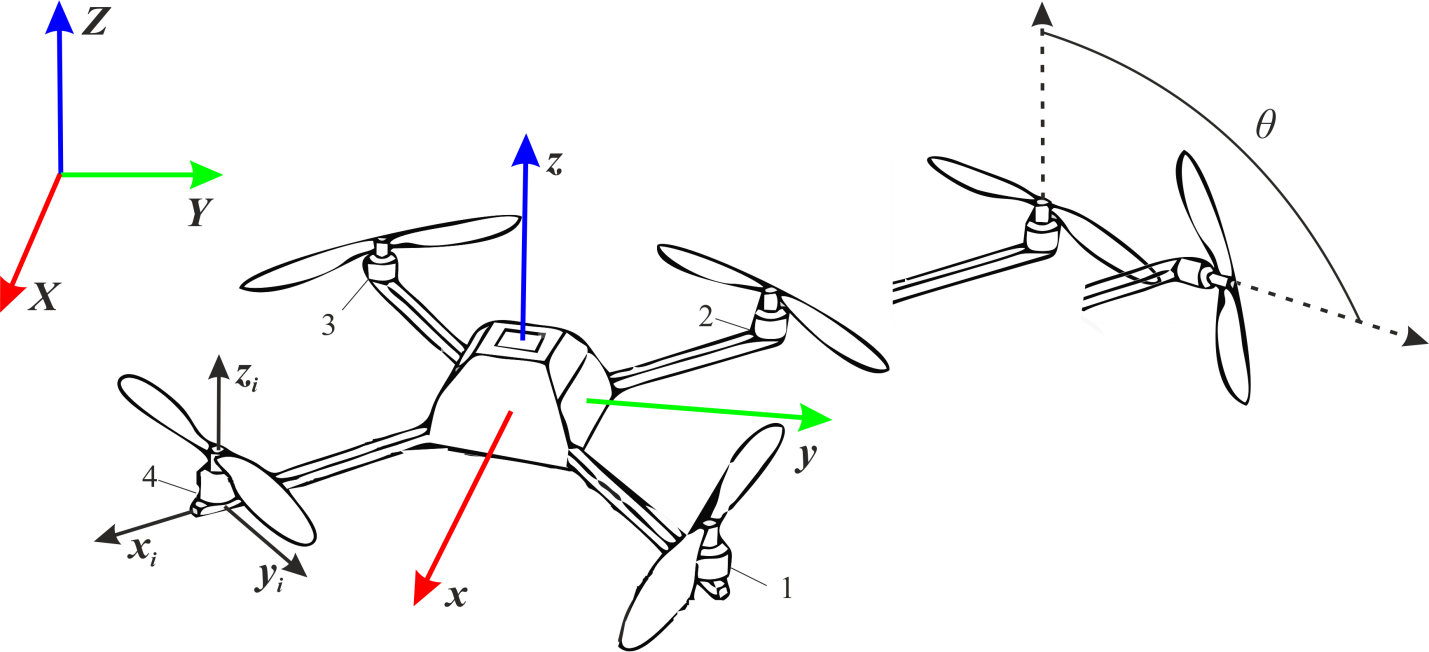
\includegraphics[scale=0.9]{tiltrotor_scheme}
	\caption{ -- Общая схема квадрокоптера с поворотными роторами}
	\label{fig:tiltrotor_scheme}
\end{figure}

\textbf{Во второй главе} рассматривается конструкция и управляемая динамика квадрокоптера с поворотными роторами.
Основным элементом конструкции БЛА является корпус, из которого выходят лучи с закрепленными на концах двигателями с пропеллерами.
Лучи расположены симметрично относительно корпуса аппарата и реализуют так называемую Х-схему.
Смежные пропеллеры имеют противоположное направление вращения; первый и третий – пропеллеры левого вращения, а второй и четвертый – правого.
Каждый из роторов может поворачиваться посредством сервопривода вокруг продольной оси луча, на котором он закреплен.
Наличие дополнительных сервоприводов усложняет модель движения БЛА \eqref{eq:common_traslational_motion} - \eqref{eq:common_rotational_motion}, делая его зависящим от текущей геометрии аппарата и скорости ее изменения

\begin{equation} \label{eq:m_traslational_motion}
M \ddot{\bm{r}} = M \bm{g}^I - \frac{1}{2} \rho C S_{\perp} |\bm{v}^I| \bm{v}^I + \sum_{i=1}^{4}{ { (-1)^{i+1} k \tilde \omega_i |\tilde \omega_i| \bm{e}^I_{z_i}}(\theta_i)},
\end{equation}

\begin{equation} \label{eq:m_final_rotational_motion}
\begin{aligned}
\bm{J}_B\dot{\bm{\Omega}}^B + \bm{\Omega}^B \times \bm{J}_B{\bm{\Omega}^B} =
&\sum_{i=1}^{4} {\bm{r}^B_i \times
	(-1)^{i+1} k \tilde \omega_i |\tilde \omega_i| \bm{e}^I_{z_i}} - \\
-\sum_{i=1}^{4} {b \tilde \omega_i |\tilde \omega_i| \bm e^{R_i}_{r_i}} +
&\sum_{i=1}^{4} q_{ B {R_i}} \circ (\bm{J}_{R_i}\dot{\bm{\omega}}^{R_i}_i + \bm{\omega}^{R_i}_i \times \bm{J}_{R_i}{\bm{\omega}^{R_i}_i}) \circ \tilde q_{ B {R_i}}
,
\end{aligned}
\end{equation}
где полная угловая скорость $\bm{\omega}^{R_i}_i$ $i$-того ротора с пропеллером
\begin{equation} \label{eq:m_prop_ang_vel}
\bm{\omega}^{R_i}_i =
q_{{R_i} B} \circ (\bm{\Omega}^B + \dot {\theta}_i \bm e^B_{r_i}) \circ \tilde {q}_{{R_i}B} +
\tilde \omega_i \bm{e}^{R_i}_{z_i}
.
\end{equation}

Считая заданной требуемую траекторию БЛА в координатном пространстве, положим целью управления обеспечение наперед заданной траектории центра масс аппарата, а также требуемой ориентации. В качестве переменных управления выберем скорости вращения пропеллеров ${\tilde \omega}_i$ и углы поворота роторов ${\theta}_i$:
\begin{equation} \label{eq:m_ctrl_out}
\begin{aligned}
&\bm{u} = (\bm \omega_u, \bm \theta_u)^T,
\\
\bm \omega_u =
(\tilde\omega_1 |\tilde\omega_1|,
\tilde\omega_2 |\tilde\omega_2|&,
\tilde\omega_3 |\tilde\omega_3|,
\tilde\omega_4 |\tilde\omega_4|)^T,
\quad
\bm \theta_u = (\theta_1, \theta_2 , \theta_3 , \theta_4 )^T.
\end{aligned}
\end{equation}
Регуляторы, обеспечивающие необходимое управление по положению и ориентации могут быть построены, как
\begin{equation} \label{eq:m_reg}
\begin{aligned}
\ddot{\bm{r}_d}(t)&=
\ddot{\bm{r}}^0(t)+\bm{K}_{r1}(\dot{\bm{r}}^0(t) - \dot{\bm{r}}(t))+\bm{K}_{r2}\delta \bm r,\\
\dot{\bm{\Omega}}_d(t)&=
\dot{\bm{\Omega}}^0(t)+\bm{K}_{\Omega1}(\bm{\Omega}^0(t)-\bm{\Omega}(t))+\bm{K}_{\Omega2}\delta\bm{q},
\end{aligned}
\end{equation}

Реализация контура управления с регуляторами (\ref{eq:m_reg}) требует обращения динамики системы, то есть определения значений всех управляющих параметров (\ref{eq:m_ctrl_out}) по выходу из регулятора (\ref{eq:m_reg}).
Для достижения этой цели преобразуем уравнения модели (\ref{eq:m_traslational_motion}), (\ref{eq:m_final_rotational_motion}).
\begin{equation} \label{eq:m_dyn}
\begin{aligned}
&\bm F(\ddot{\bm r}_d, \dot{\bm r}, q) = k F_{thr} (\bm \theta_u) \bm \omega_u,\\
&\bm T(\dot{\bm \Omega}_d, \bm\Omega) = \Big(
kLT_{thr}(\bm\theta_u) - bT_{aero}(\bm\theta_u)
\Big)
\bm \omega_u.
\end{aligned}
\end{equation}

Система (\ref{eq:m_dyn}) недоопределена и нелинейна относительно компонент $\bm \theta_u$, что значительно затрудняет ее аналитическое решение. Доопределим систему, используя выражения для распределения вертикальных составляющих сил и моментов между парами двигателей, расположенных на параллельных лучах
\begin{equation} \label{eq:m_dyn_balance_1}
\begin{aligned}
&k \tilde\omega_1 |\tilde\omega_1| c_1 + k \tilde\omega_3 |\tilde\omega_3| c_3 =
\frac{1}{2} \bm F_z + \varepsilon_F,
\\
&\tilde\omega_1 |\tilde\omega_1| (bc_1 - kLs_1)
+ \tilde\omega_3 |\tilde\omega_3| (bc_3 - kLs_3) =
\frac{1}{2} \bm T_z + \varepsilon_T,
\end{aligned}
\end{equation}

\begin{equation} \label{eq:m_dyn_balance_2}
\begin{aligned}
&k \tilde\omega_2 |\tilde\omega_2| c_2 + k \tilde\omega_4 |\tilde\omega_4| c_4 =
-\frac{1}{2} \bm F_z + \varepsilon_F,
\\
&\tilde\omega_2 |\tilde\omega_2| (bc_2 + kLs_2)
+ \tilde\omega_4 |\tilde\omega_4| (bc_4 + kLs_4) =
\frac{1}{2} \bm T_z - \varepsilon_T,
\end{aligned}
\end{equation}
где $\varepsilon_F$ и $\varepsilon_F$ -- балансировочные параметры.
Полученная система уравнений (\ref{eq:m_dyn}), (\ref{eq:m_dyn_balance_1}) имеет аналитическое решение:
\begin{equation} \label{eq:m_dyn_resolve}
\begin{aligned}
&\tilde\omega_i |\tilde\omega_i| =
\frac{(-1)^{i+1}}{2kL}\sqrt{
	A^2_i + 
	B^2_i
},
\\
\phantom{}
\\
&\theta_i = 
2 \text{arctg} \Bigg[(-1)^{i+1}	
\frac{A_i -
	\sqrt{
		A^2_i + 
		B^2_i
}}
{B_i}
\Bigg],
\end{aligned}
\end{equation}
где $A_i = A_i(\bm F, \bm T, \varepsilon_F, \varepsilon_T)$
и
$B_i = B_i(\bm F, \bm T, \varepsilon_F, \varepsilon_T)$
-- скалярные функции, куда линейно входят компоненты левой части уравнений динамики \eqref{eq:m_dyn}
$\bm F(\ddot{\bm r}_d, \dot{\bm r}, q)$
и
$\bm T(\dot{\bm \Omega}_d, \bm\Omega)$.
Таким образом, полученное решение связывает выход регулятора с управляющими параметрами при наличии обратной связи, а именно известных текущих координате $\bm r^I$, скорости $\bm v^I$, ориентации $q_{IB}$ и угловой скорости $\bm \Omega^B$.

Анализ решения \eqref{eq:m_dyn_resolve} позволяет ограничить выход регулятора \eqref{eq:m_reg} таким образом, чтобы компоненты вектора управляющих воздействий не выходили за пределы заданных значений 
\begin{equation} \label{eq:m_limits_init}
\begin{aligned}
&0< (-1)^{i+1} \tilde \omega_i |\tilde\omega_i| < \tilde \omega_{max}^2,
\\
&|\theta_i| < \theta_{max} < \pi,
\end{aligned}
\end{equation}
что позволяет учесть ограничения на физические параметры исполнительных органов системы управления.

Затем рассматривается сценарий потери аппаратом двух смежных двигателей. Экстренное управление БЛА является немаловажной частью исследований их управляемой динамики, и данной теме посвящено немало работ. В последних из них авторам удалось добиться возможности продолжения миссии квадрокоптера стандартной конструкции с одним вышедшим из строя двигателем на высокой скорости и показать, что успешная посадка аппарата возможна даже при наличии всего двух работающих двигателей, расположенных на противолежащих лучах аппарата. Подобные исследования проводились также для квадрокоптеров с поворотными роторами, где дополнительные исполнительные органы системы управления, а именно сервоприводы, изменяющие направления тяги оставшихся двигателей, способны частично компенсировать потерю управляемости БЛА вследствие потери одного двигателя.
Среди нерассмотренных сценариев остается потеря двух смежных двигателей, что вполне может произойти, например, при лобовом столкновении с препятствием, таким как стена здания.
В работе показано, что наличие поворотных роторов может спасти аппарат от неконтролируемого падения и обеспечить мягкую посадку при потере двух смежных двигателей.

\textbf{Третья глава} посвящена реализации обратных связей в контуре управления. Для реализации обратных связей в контуре управления необходимо обеспечить оценку текущего положения, скорости, кватерниона ориентации и угловой скорости БЛА. Получить данные оценки можно с помощью стандартного набора бортовых датчиков, обычно включающего в себя спутниковую систему глобального позиционирования, цифровой барометрический датчик давления, трехосевые электромеханические акселерометр и гироскоп, а также магнитный компас. Однако в связи с высокими требованиями к массово-габаритным параметрам бортовой системы навигации для небольших летательных аппаратов бортовые измерения имеют ограничения по качеству. Высокий уровень шума побуждает использовать алгоритмы оценки состояния, способные значительно понизить его уровень.

Для выбора подходящего алгоритма фильтрации было проведено исследование, где были рассмотрены  алгоритмы расширенного фильтра Калмана (extended Kalman filter, EKF) и несколько вариантов реализации сигма-точечного фильтра Калмана (unscented Kalman filter, UKF). Приводится описание принципов работы EKF, UKF, а также одной из частных реализаций сигма-точечного фильтра -- кубатурного фильтра Калмана (cubature Kalman filter, CKF) и описаны особенности применения этих алгоритмов для оценки состояния квадрокоптера с поворотными роторами.

Для сравнения производительности методов проведены вычислительные эксперименты.
Предложенные во второй главе алгоритмы использовались для управления БЛА, в качестве целевых траекторий выбраны трехмерные кривые в пространстве, параметры которых генерировались случайным образом в известных пределах. В качестве параметра, определяющего производительность фильтров,
выбрано среднеквадратичное отклонение компонент вектора оценки состояния от результатов интегрирования уравнений движения.
Для исключения влияния параметров конкретной целевой траектории на результаты эксперимента среднеквадратичное отклонение усредняется по 100 различным траекториям.
На графике ниже (рис. \ref{fig:est_cmpr}) представлена зависимость усредненного среднеквадратичного отклонения от интервала проводимых измерений $T_N = N\delta$ для высоты, вертикальной скорости, угла рысканья и скорости его изменения.

\begin{figure}[H]
	\begin{minipage}[h]{0.49\linewidth}
		\center{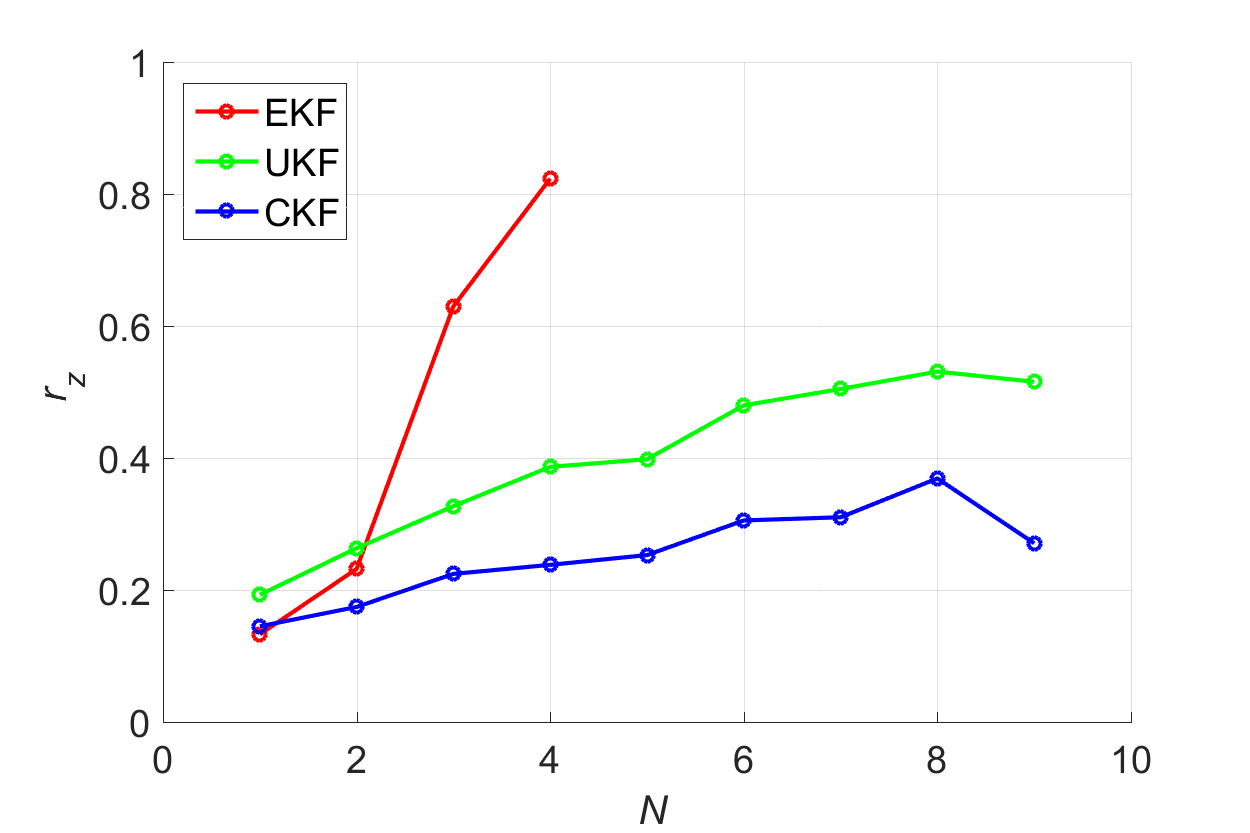
\includegraphics[height=0.2\textheight]{estcmpr_1} \\ а)}
	\end{minipage}
	\hfill
	\begin{minipage}[h]{0.49\linewidth}
		\center{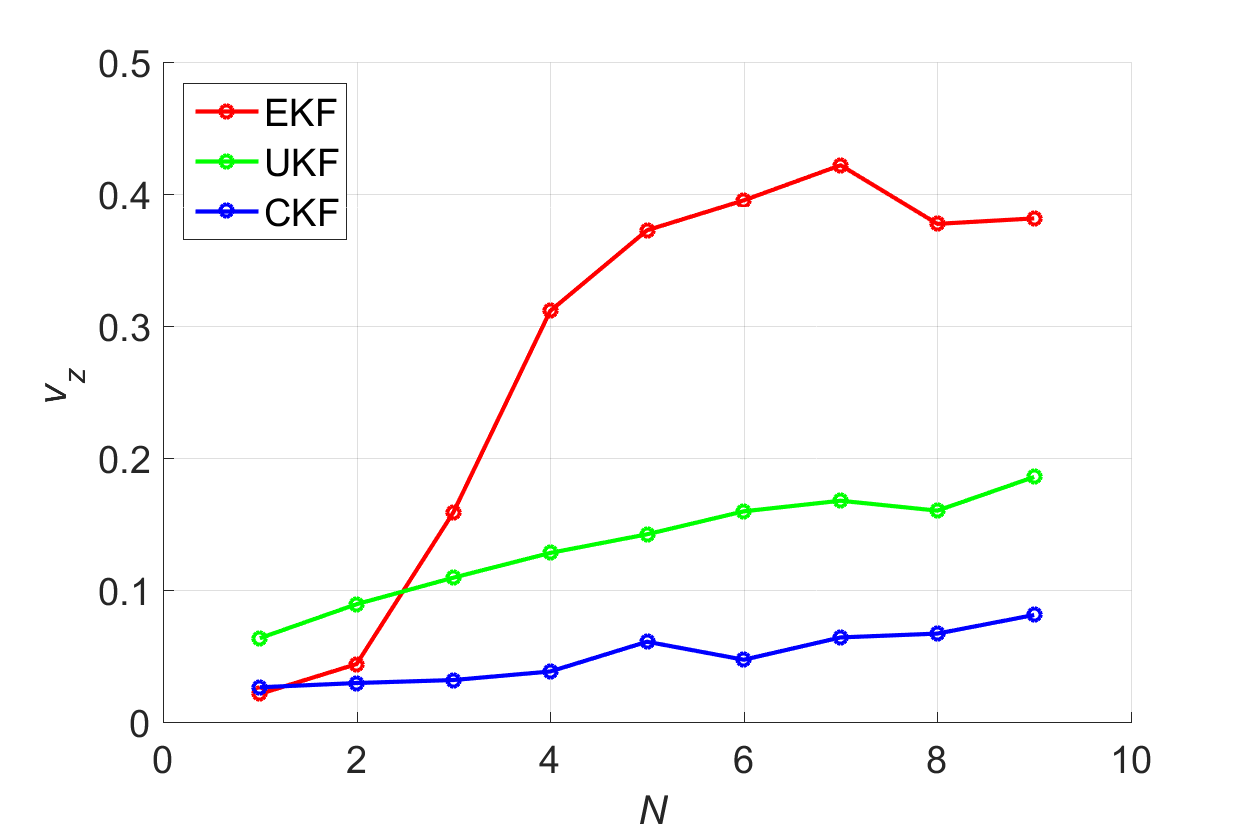
\includegraphics[height=0.2\textheight]{estcmpr_2} \\ б)}
	\end{minipage}
	\\
	\begin{minipage}[h]{0.49\linewidth}
		\center{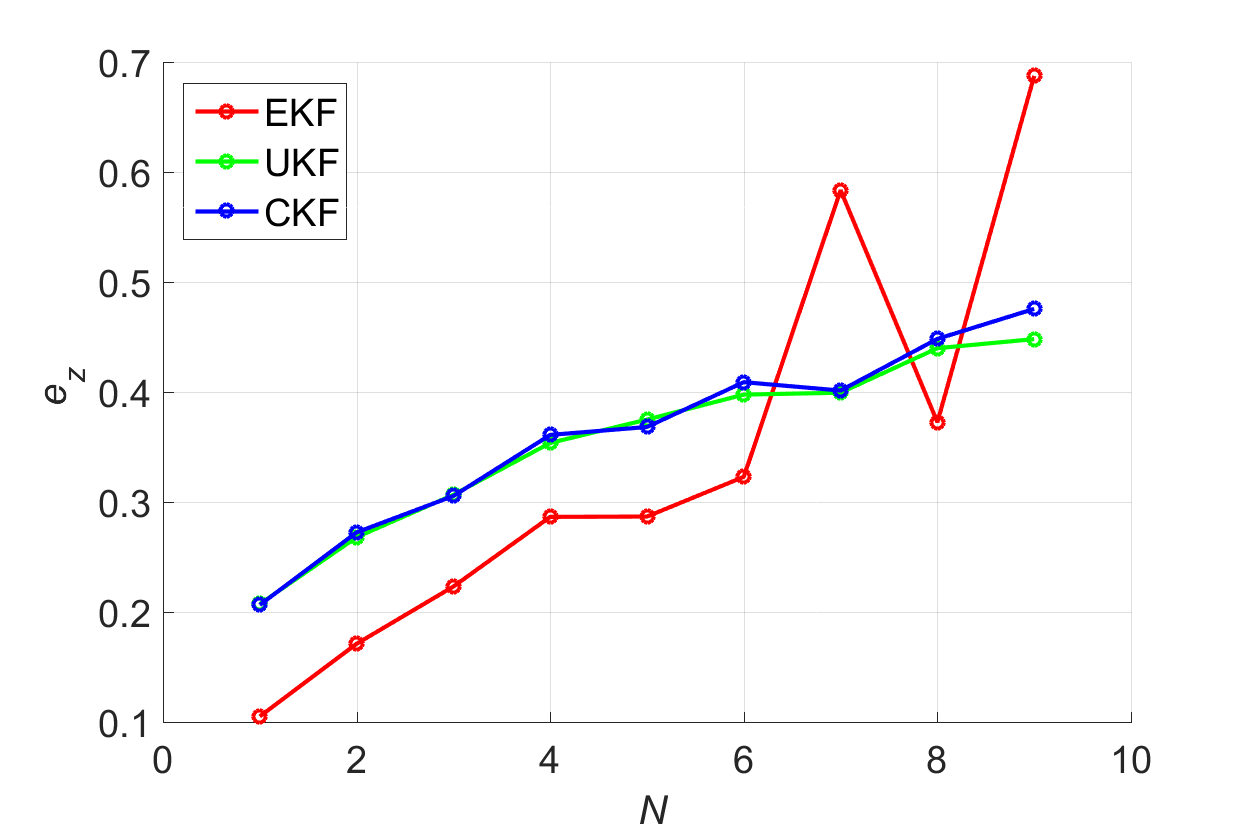
\includegraphics[height=0.2\textheight]{estcmpr_3} \\ а)}
	\end{minipage}
	\hfill
	\begin{minipage}[h]{0.49\linewidth}
		\center{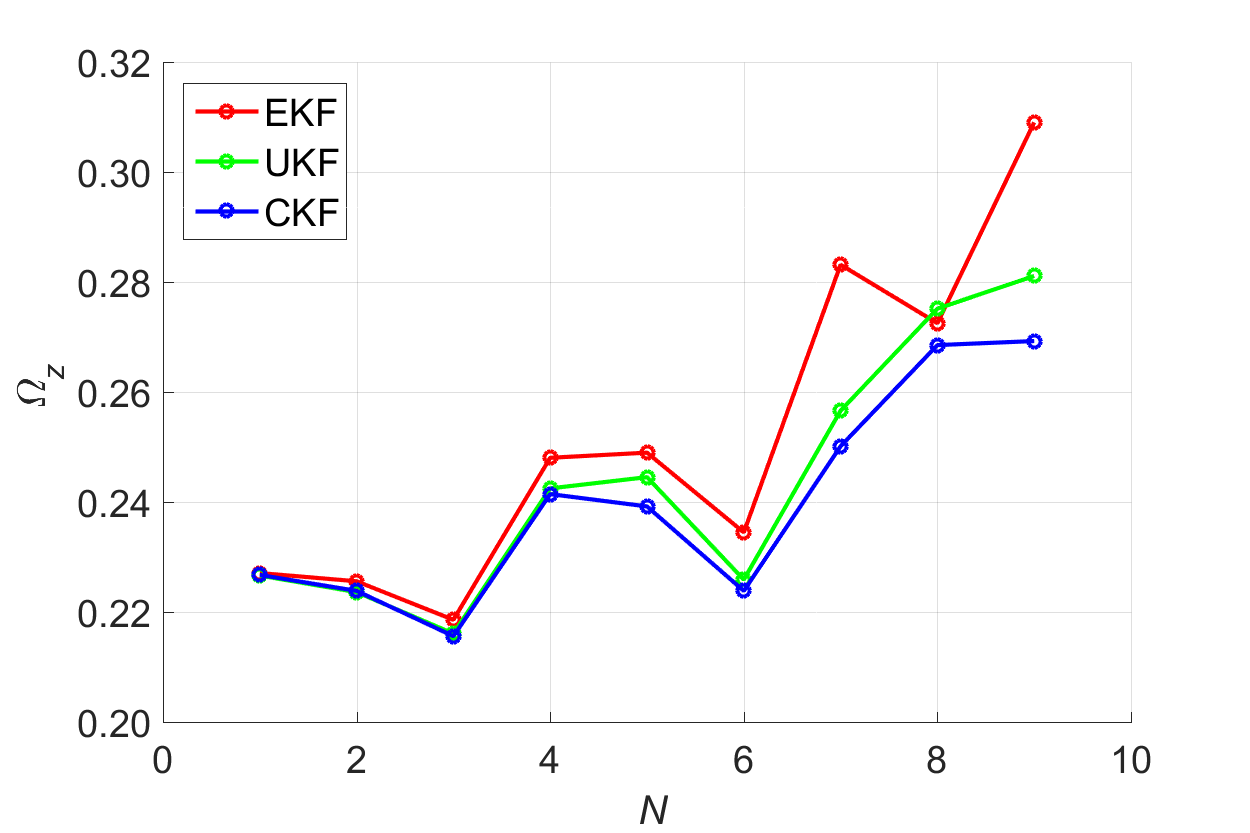
\includegraphics[height=0.2\textheight]{estcmpr_4} \\ б)}
	\end{minipage}
	\caption{Сравнение производительности алгоритмов фильтрации}
	\label{fig:est_cmpr}
\end{figure}

Качество оценки вектора состояния зависит от величины интервала работы фильтра --
снижение частоты измерений ведет к ухудшению параметров оценки.
Наиболее низкую производительность на больших интервалах измерений показывает расширенный фильтр Калмана:
уже для $N>2$ ошибки оценки состояния в нескольких случаях выходят за рамки допустимых,
а при $N \geq 5$ оценка положения становится некорректной.
Производительность сигма-точечного и кубатурного фильтров Калмана с ростом $N$ также падает,
но не настолько заметно.
Сравнительный анализ результатов UKF и CKF показал, что CKF-алгоритм производит более точную оценку состояния
в большинстве рассматриваемых случаев и является более устойчивым к повышению интервала измерений.
Таким образом для системы управления квадрокоптером с поворотными роторами был выбран кубатурный фильтр Калмана.

\textbf{В четвертой главе} представлены результаты вычислительных экспериментов. 
В первом эксперименте аппарат должен выполнить наблюдение за подвижным объектом, летя неподалеку от него и ориентируя камеру, установленную спереди, так, чтобы объект находился в центре полученного изображения. Выбраны параметры, соответствующие небольшому квадрокоптеру, способному нести на борту дополнительную нагрузку в виде камеры высокого разрешения (Таблица \ref{tb:params_table}).
Рассчитаны ограничения на выходы регулятора
для 
$\tilde \omega_{max}$ = 1140 рад/с,
$\theta_{max}$ = ${\pi}/{3}$ рад.
\begin{table}[h!]
	\centering
	\caption{ -- Параметры модели}\label{tb:params_table} 
	\begin{tabular}{lcl}
		\hline
		Параметр & Обозначение & Значение  \\\hline
		Общая масса & $M$ & 2 кг  \\
		Тензор инерции корпуса & $\bm J_B$ & $diag(2,\ 2,\ 4)\cdot{10^{-2}}$ кг$\cdot$м$^2$  \\
		Тензор инерции ротора & $\bm J_R$ & $diag(2,\ 2,\ 1)\cdot{10^{-5}}$ кг$\cdot$м$^2$  \\
		Миделево сечение корпуса & $S_{\perp}$ & 0,12 м$^2$ \\
		Луч & $L$ & 0,25 м \\
		Аэродинамический коэффициент & $C$ & 1,05\\
		Аэродинамический коэффициент & $k$ & 1,13$\cdot 10^{-5}$ Н$\cdot$с$^2\cdot$рад$^{-2}$ \\		
		Аэродинамический коэффициент & $b$ & 1,5$\cdot 10^{-6}$ Н$\cdot$м$\cdot$с$^2\cdot$рад$^{-2}$ \\		
		Максимальные обороты & $\tilde \omega_{max}$ & 1140 рад/с \\		
		Максимальный угол & $\theta_{max}$ & ${\pi}/{3}$ рад \\
		Константа балансировки & $\varepsilon_\tau$ &6 Н$\cdot$м \\
		\hline
	\end{tabular}
\end{table}
Траектория БЛА и наблюдаемого объекта изображены на рисунке \ref{fig:mau_traj}.
\begin{figure}[H]
	\centering
	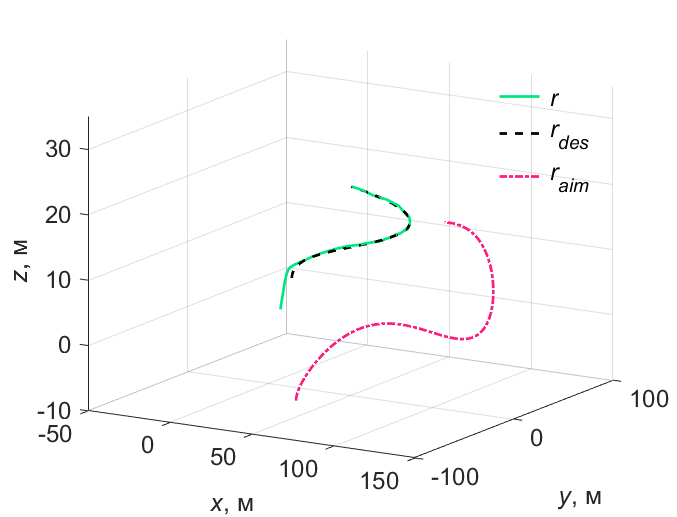
\includegraphics[width=14cm]{traj.png}
	\caption{ -- Траектория БЛА и объекта наблюдения}
	\label{fig:mau_traj}
\end{figure}

На рисунке \ref{fig:mau_errors}, на графиках слева, изображены ошибки ориентации по углам крена, тангажа и рысканья,
а справа -- ошибки положения  квадрокоптера по осям $X$, $Y$ и $Z$.
Ошибки по каждому из углов ориентации после стабилизации не превышают одного градуса.
После выхода аппарата на целевую траекторию максимальное абсолютное отклонение от траектории составило 30 см.
\begin{figure}[H]
	\centering
	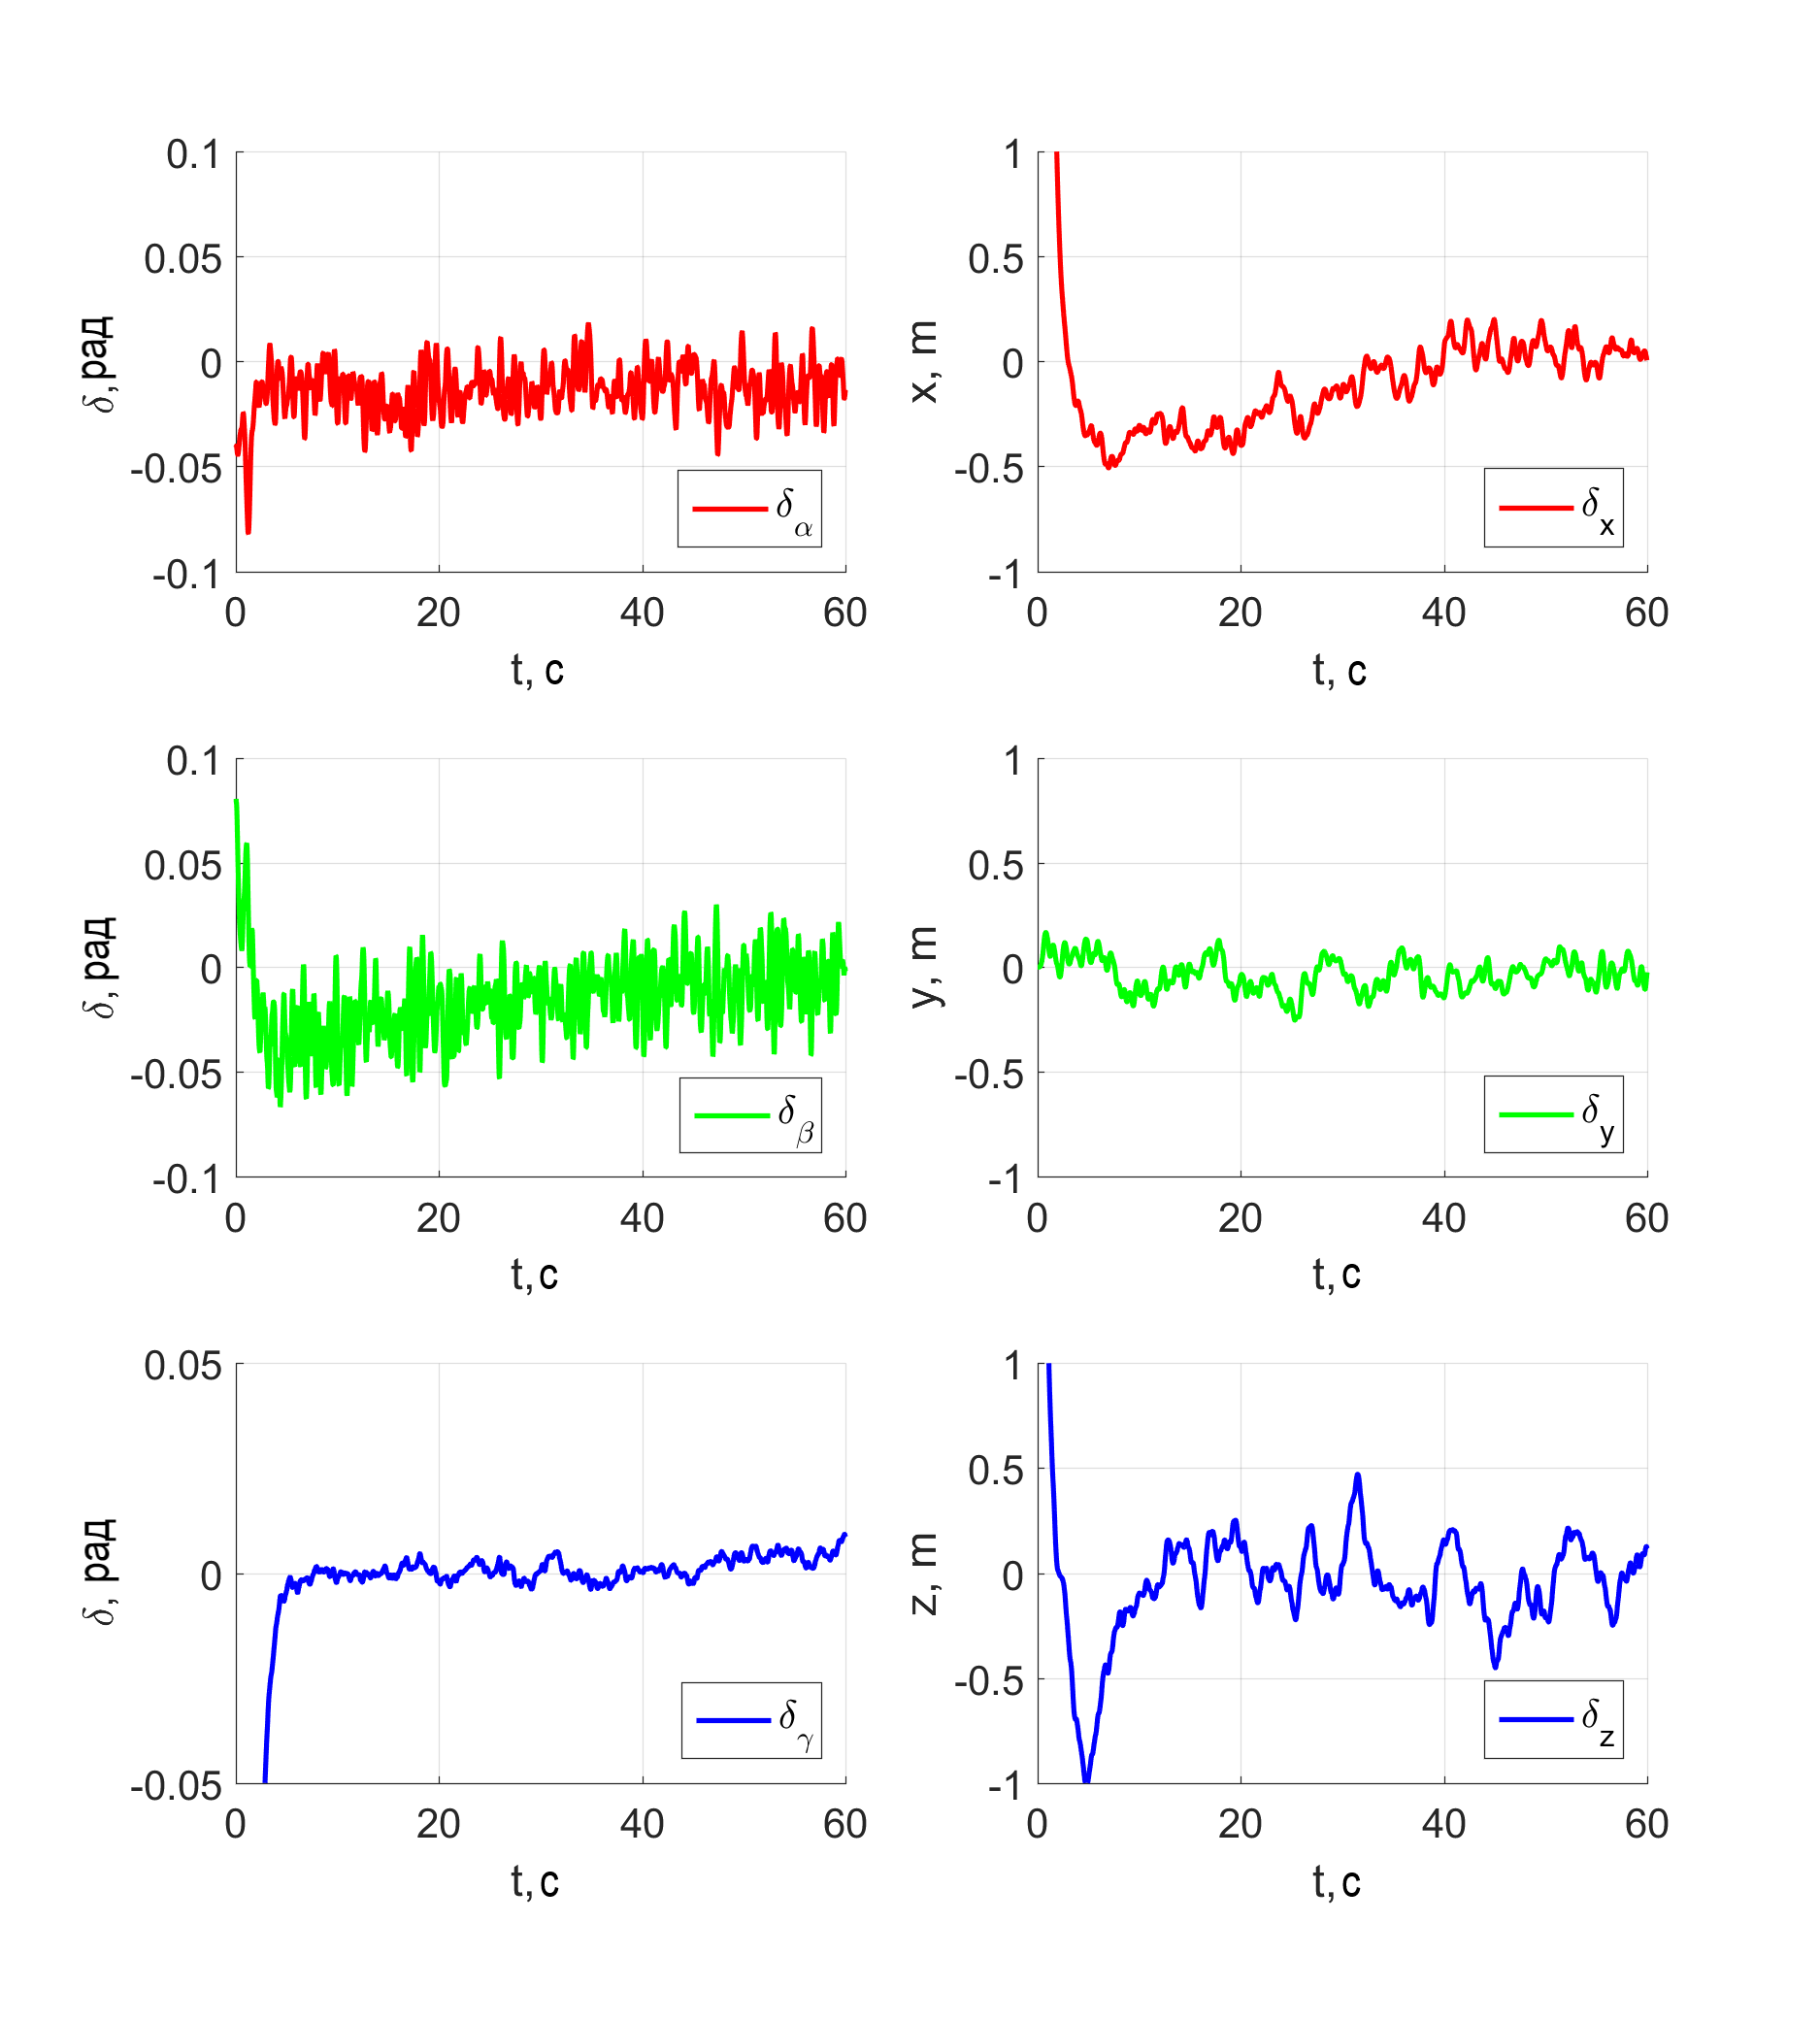
\includegraphics[width=14cm]{errors_rows.png}
	\caption{ -- Отклонение параметров движения БЛА от целевых значений}
	\label{fig:mau_errors}
\end{figure}

На рисунке \ref{fig:mau_cam} можно проследить за траекторией наблюдаемого объекта на записи, которою можно сделать с помощью передней камеры.
Видно, что в начальный момент времени объект находится вне зоны видимости, затем перемещается в центр экрана и далее на протяжении всего времени маневра ось визирования камеры отклоняется от направления на объект не более чем на 1$^\circ$.
\begin{figure}[H]
	\centering
	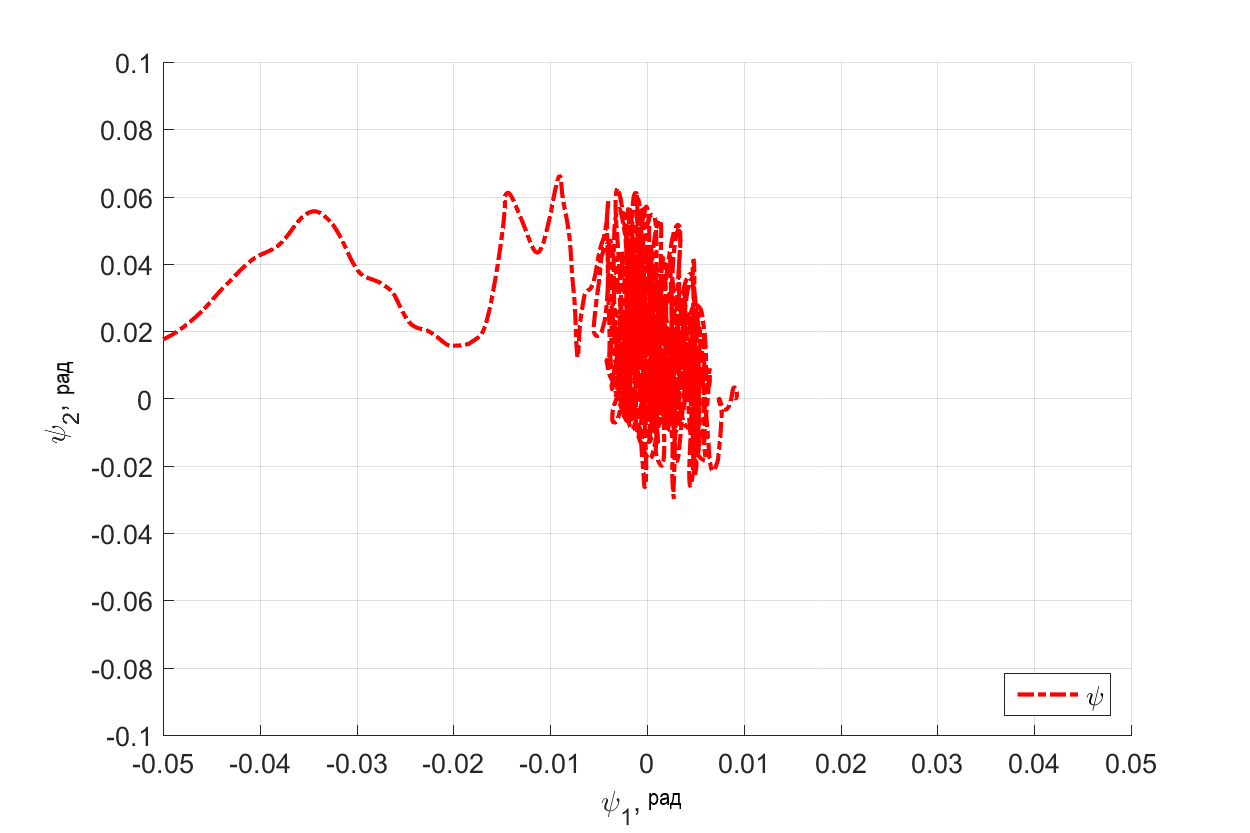
\includegraphics[width=14cm]{camera.png}
	\caption{ -- Траектория объекта на записи}
	\label{fig:mau_cam}
\end{figure}
Рисунок \ref{fig:mau_est} демонстрирует производительность кубатурного фильтра Калмана. Слева приведен график ошибки оценки угла крена и его прямых измерений, справа – оценка положения по оси $X$ и его прямые измерения.
Алгоритмы фильтрации позволили значительно понизить уровень шума измерений.
\begin{figure}[H]
	\centering
	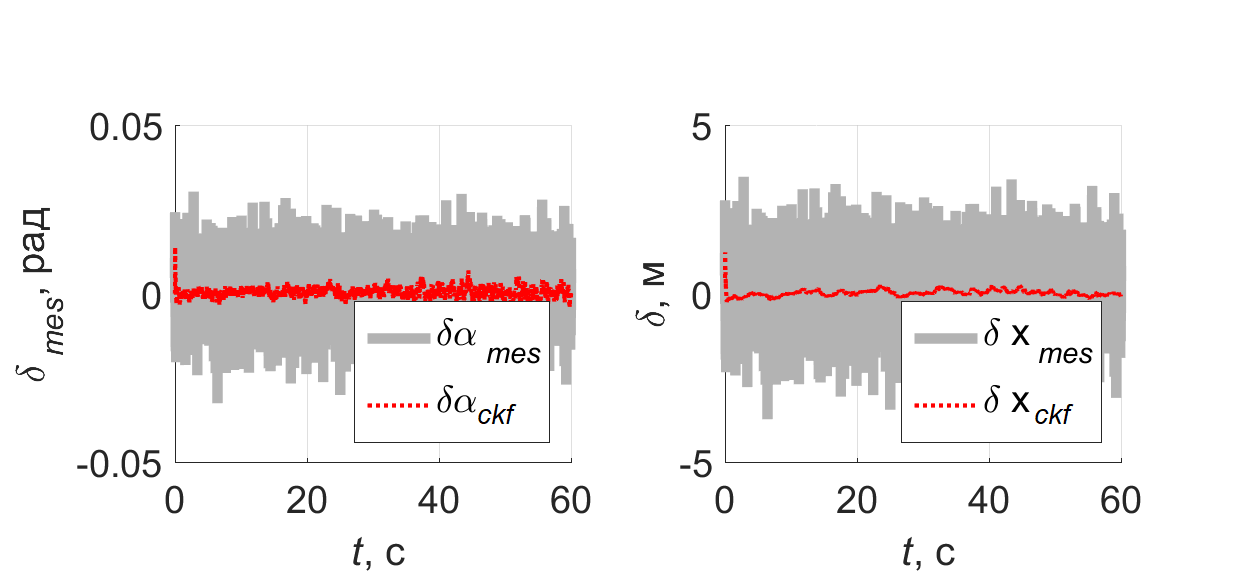
\includegraphics[width=14cm]{ckf_perf_raws_cut.png}
	\caption{ -- Ошибка оценки состояния и прямых измерений}
	\label{fig:mau_est}
\end{figure}

На графиках, изображенных на рисунке \ref{fig:mau_ctrl_out} представлены компоненты вектора управляющих параметров, которые лежат внутри ограниченной предельными значениями области.

\begin{figure}[H]
	\centering
	\subfloat{%
		\subfloat[]{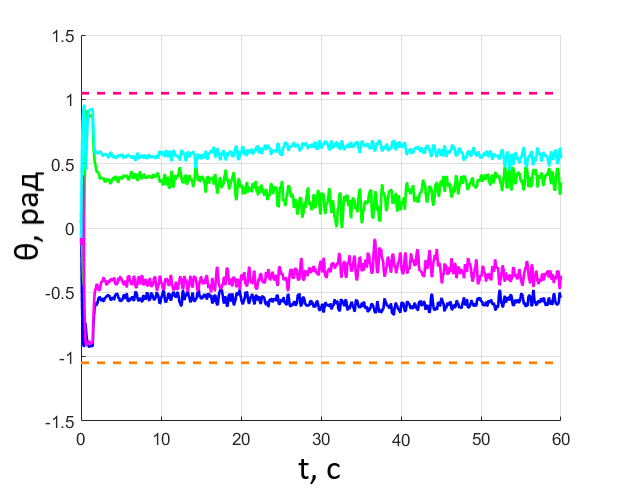
\includegraphics[clip,width=0.49\columnwidth]{rotor_angles}}%
		\subfloat[]{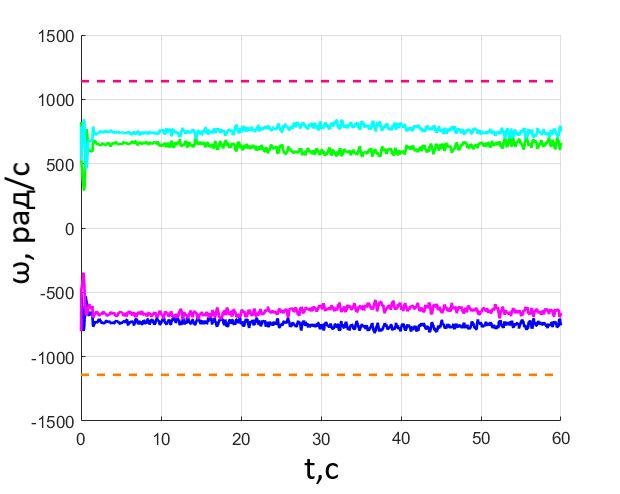
\includegraphics[clip,width=0.49\columnwidth]{rotor_rates}}%
	}
	
	\caption{ -- Управляющие параметры}
	\label{fig:mau_ctrl_out}
	
\end{figure}


В результате эксперимента мы оценили способность БЛА с поворотными роторами справляться со сложными маневрами, где необходимо независимо управлять ориентацией и положением аппарата. Квадрокоптер быстро вышел на целевую траекторию и успешно отслеживал ее, ориентируя бортовую камеру таким образом, чтобы объект наблюдения всегда оставался в центре изображения.

Во втором эксперименте рассматривается сценарий отказа двух смежных двигателей. Для возможности применения системы экстренного управления необходим значительный запас тяги двигателей и широкие пределы отклонений сервоприводов
\begin{equation}
\begin{aligned}
&\tilde{\omega}_{max} = 1318 рад/c,
\\
&\theta_{max} = \pi.
\end{aligned}
\end{equation}

В начальный момент времени аппарат находится на высоте 25 метров недалеко от точки взлета.
При отказе двигателей начинается переход в режим экстренного управления.
За время менее 5 секунд высота БЛА упала более чем на 15 метров, но затем, когда аппарат стабилизировал свою ориентацию около целевых значений, падение прекратилось и аппарат приступил к плавному снижению со скоростью около 0,5 метров в секунду с одновременным движением в сторону места своего запуска. По истечении 30 секунд квадрокоптер стабилизировал свое положение около точки взлета. На рисунке \ref{fig:em_coords} представлены параметры движения мультироторного робота в процессе экстренной посадки. Слева изображены графики компонент векторной части кватерниона ориентации корпуса, справа -- проекции координат центра масс БЛА на оси инерциальной системы отсчета.
\begin{figure}[H]
	
	\centering
	\subfloat[крен]{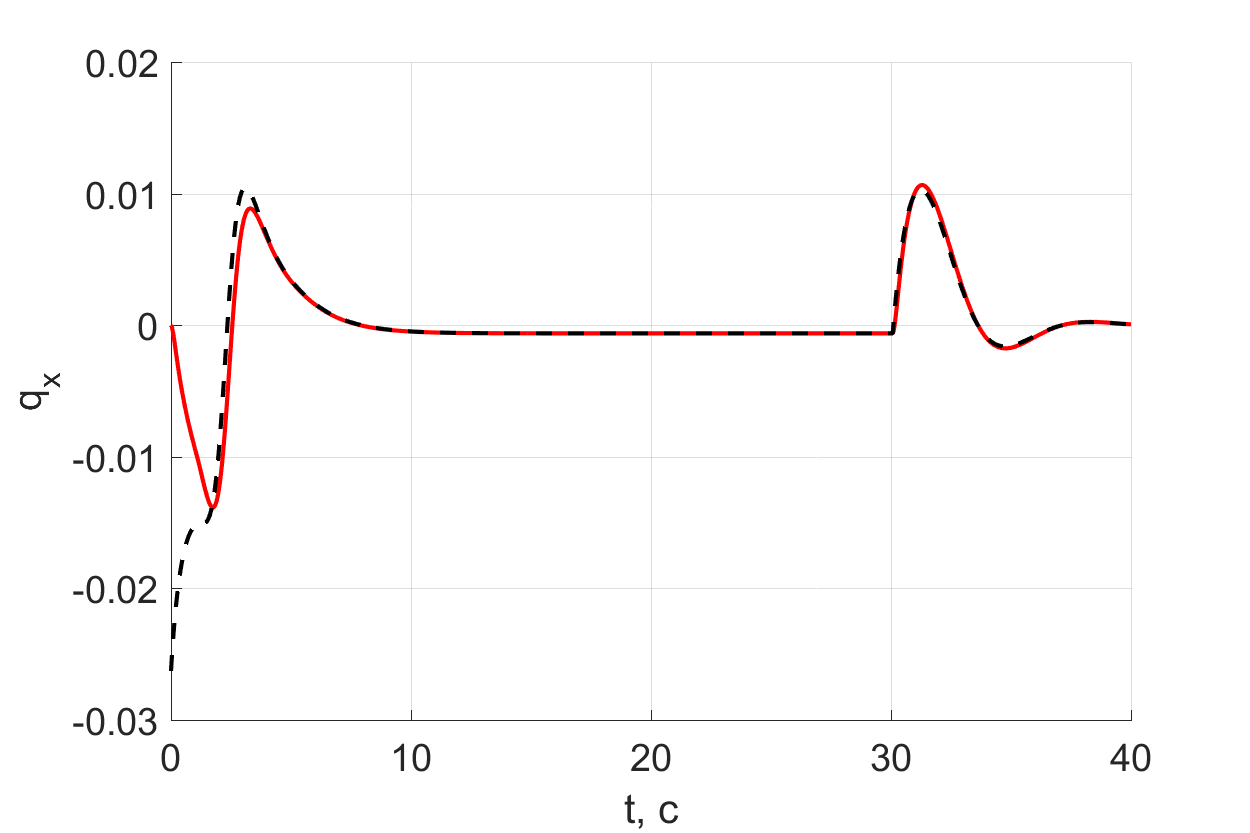
\includegraphics[width=7cm]{em/roll}}\hfil
	\subfloat[координата x]{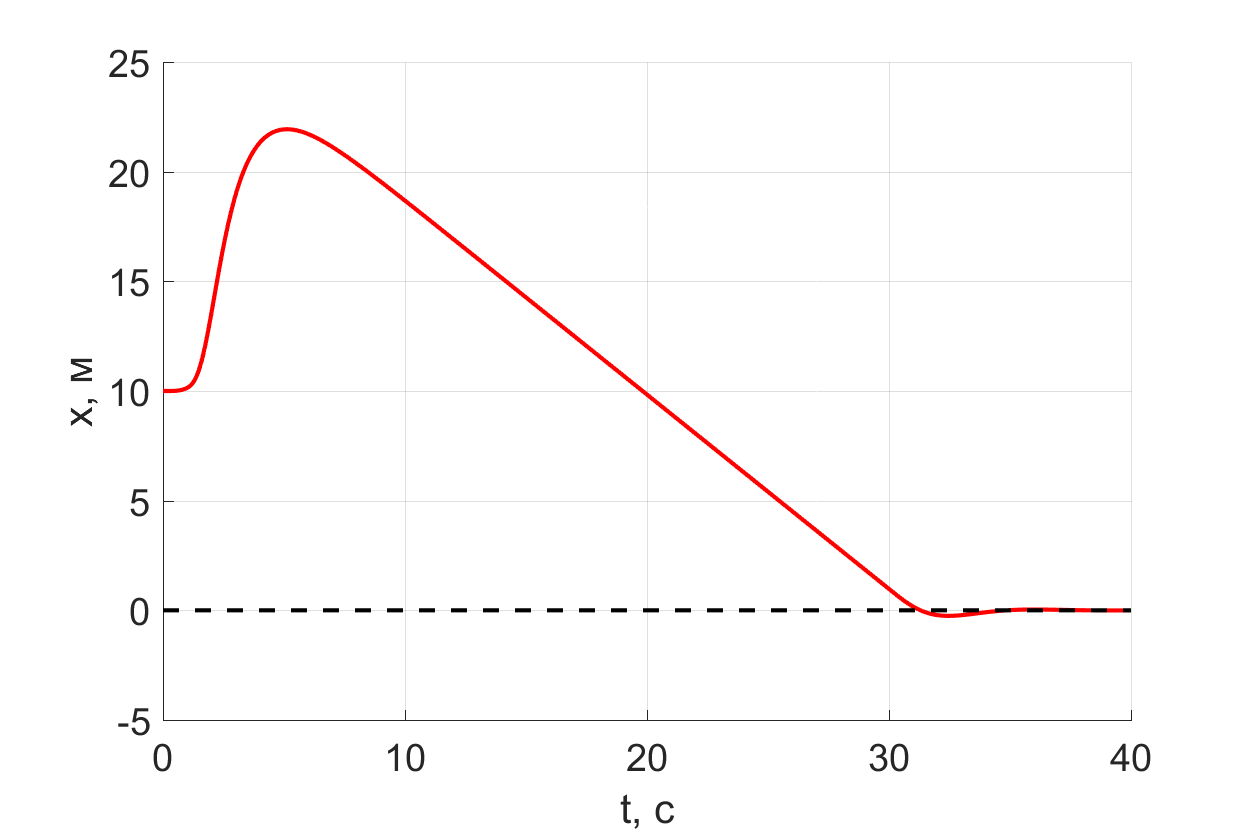
\includegraphics[width=7cm]{em/x}}
	
	\subfloat[тангаж]{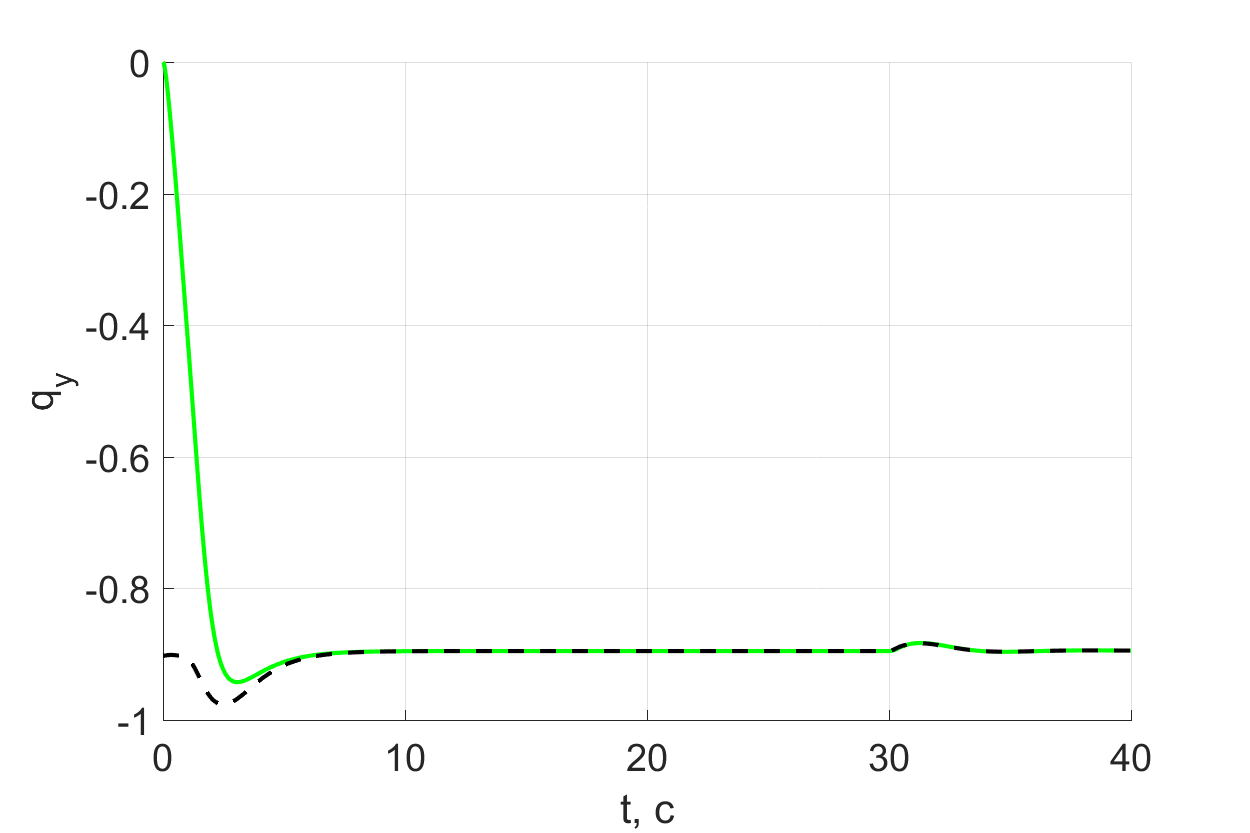
\includegraphics[width=7cm]{em/pitch}} \hfil 
	\subfloat[координата y]{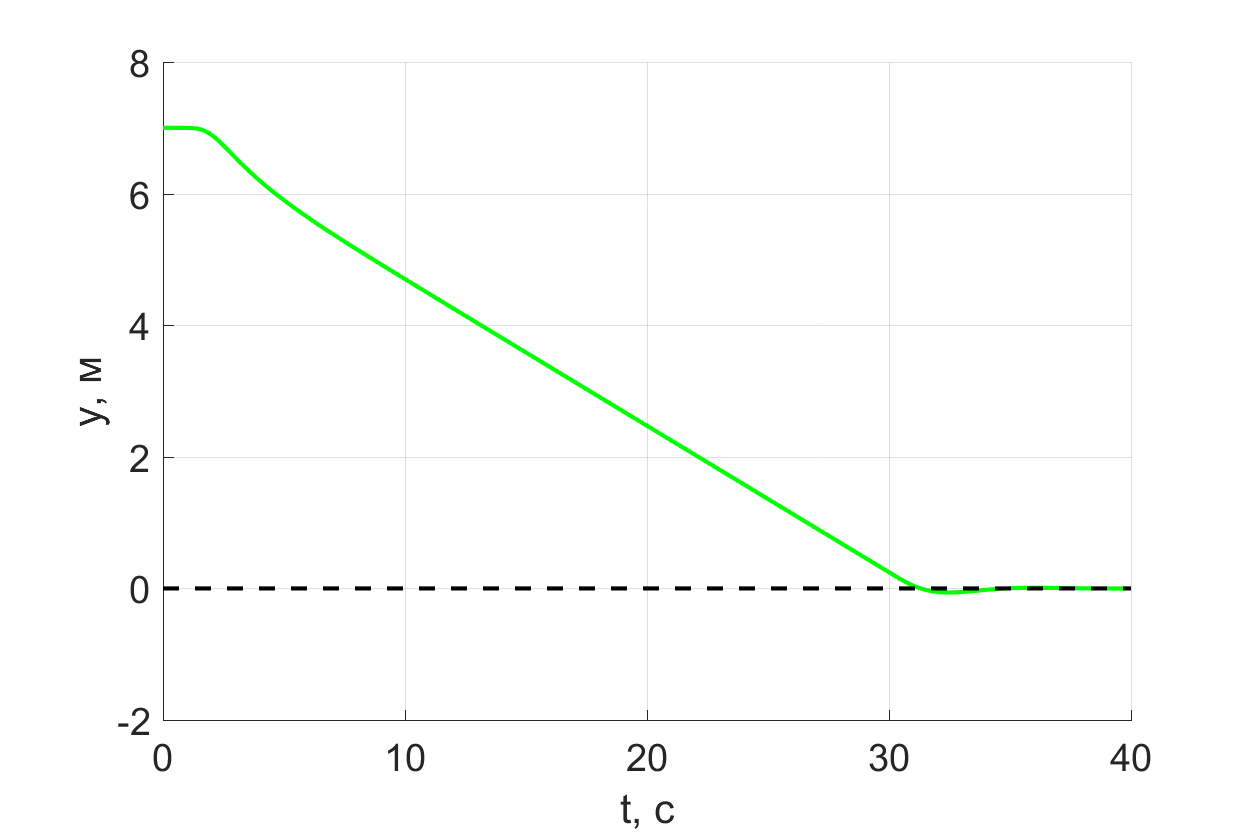
\includegraphics[width=7cm]{em/y}}  
	
	\subfloat[рысканье]{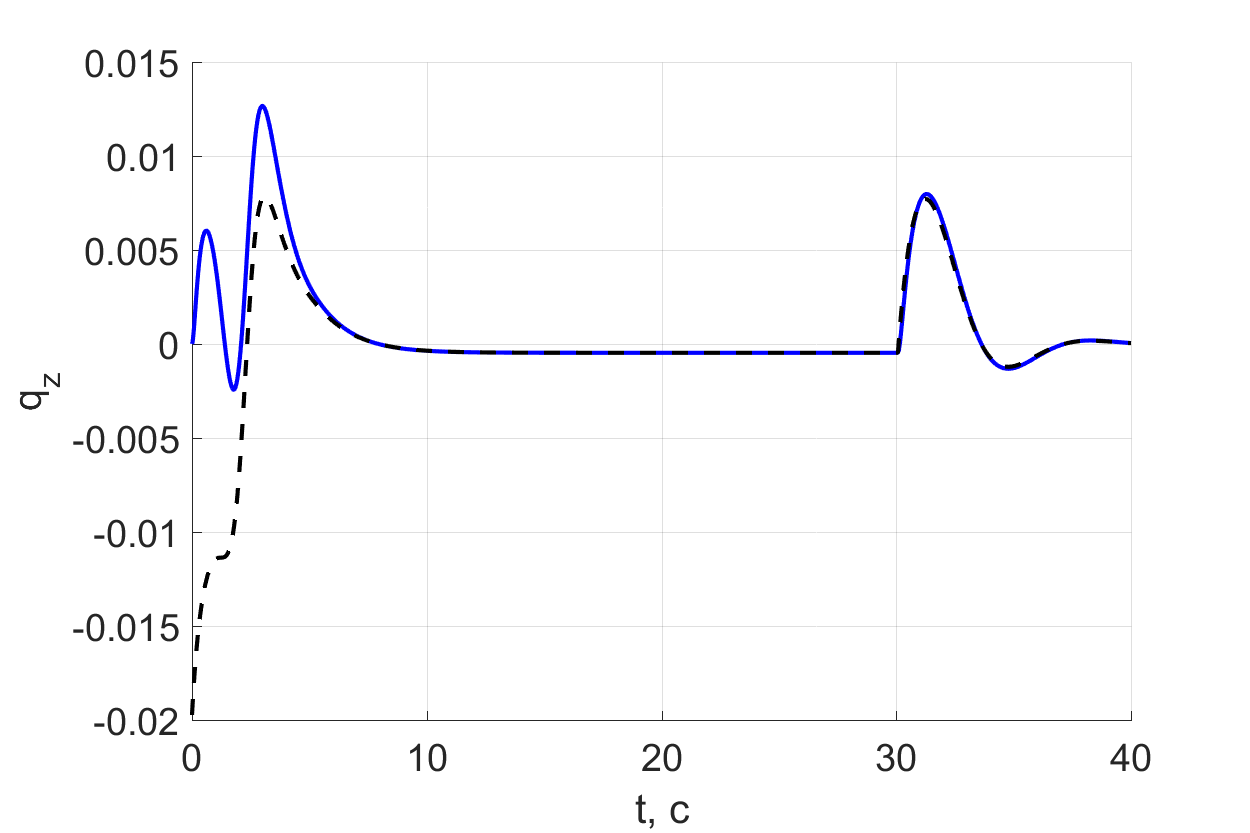
\includegraphics[width=7cm]{em/yaw}}\hfil
	\subfloat[координата z]{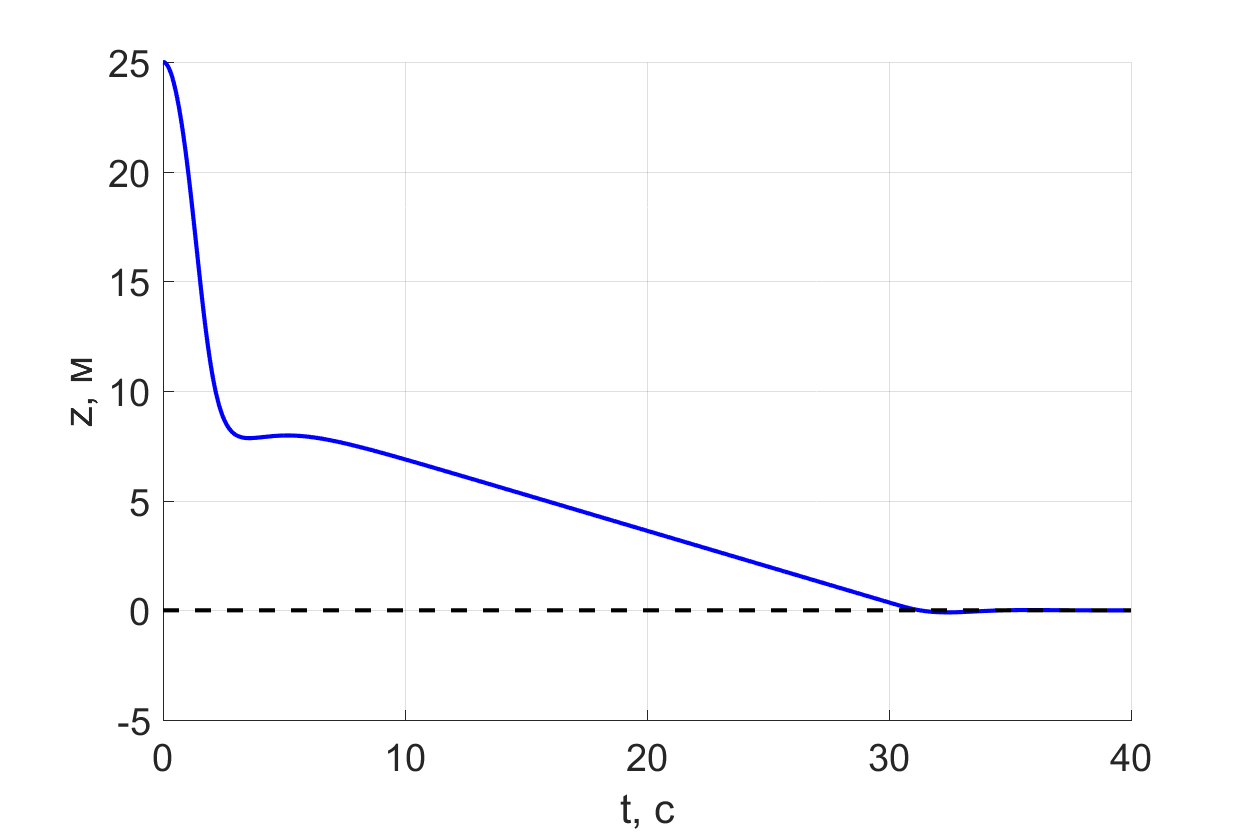
\includegraphics[width=7cm]{em/z}}
	\caption{ -- Параметры движения БЛА при экстренной посадке}
	\label{fig:em_coords}
\end{figure}

Таким образом было показано, что БЛА с поворотными роторами при соблюдении некоторых требований к параметрам исполнительных органов системы управления способен продолжить свое движение после отказа двух смежных двигателей.

\textbf{В заключении} приводятся основные результаты диссертационной работы:
\begin{enumerate}
	\item Разработана математическая модель управляемой динамики квадрокоптера с поворотными роторами с учетом сил и моментов, действующих на все составные части системы;
	\item  Получено аналитическое решение задачи обратной динамики БЛА с поворотными роторами;
	\item Синтезирован контур управления квадрокоптером с поворотными роторами для независимого управления положением и ориентацией; 
	\item Разработан алгоритм для учета физических ограничений, накладываемых на исполнительные органы системы управления;
	\item Разработан алгоритм для идентификации основных параметров модели;
	\item Разработаны алгоритмы оценки состояния БЛА с поворотными роторами и проведен их сравнительный анализ.
	\item Разработаны алгоритмы экстренного управления квадрокоптером с поворотными роторами в случае отказа двух смежных двигателей.
\end{enumerate}

	\sloppy
	\printbibliography
\end{document}

